%%%  کلاس AUTthesis، نسخه آبان 1397
%%%   دانشگاه صنعتی امیرکبیر                 http://www.aut.ac.ir
%%%  تالار گفتگوی پارسی‌لاتک،       http://forum.parsilatex.com
%%%   آپدیت شده در آبان 95
%%%   پشتیبانی و راهنمایی          badali_farhad@yahoo.com
%%%
%%%   بازبینی و اصلاح شده در آبان ماه 1397
%%%  Tested via TeXstudio in TeXlive 2014-2018.
%%%

%-----------------------------------------------------------------------------------------------------
%        روش اجرا.: 2 بار F1 ، 2 بار  F11(به منظور تولید مراجع) ، دوبار Ctrl+Alt+I (به منظور تولید نمایه) و IIدو بار F1 -------> مشاهده Pdf
%%%%%%%%%%%%%%%%%%%%%%%%%%%%%%%%%%%%%%%%%%%%%%%%%%%%%%
%   TeXstudio as your IDE
%%  برای compile در TeXstudio تنها کافی است منوی Options->Configure TeXstudio را زده و در پنجره Configure TeXstudio در بخش Build گزینه Default Compiler را به XeLaTeX تغییر دهید. سند شما به راحتی compile خواهد شد.
%   F1 & F5 : Build & view
%   F6      : Compile
%   F7      : View
%   --------------
%%%%%%%%%%%%%%%%%%%%%%%%%%%%%%%%%%%%%%%%%%%%%%%%%%%%%%
%        اگر قصد نوشتن رساله دکتری را دارید، در خط زیر به جای msc،
%      کلمه phd را قرار دهید. کلیه تنظیمات لازم، به طور خودکار، اعمال می‌شود.
%%% !TEX TS-program = XeLaTeX
\documentclass[oneside,bsc,12pt]{AUTthesis}
%       فایل commands.tex را حتماً به دقت مطالعه کنید؛ چون دستورات مربوط به فراخوانی بسته زی‌پرشین 
%       و دیگر بسته‌ها و ... در این فایل قرار دارد و بهتر است که با نحوه استفاده از آنها آشنا شوید. توجه شود برای نسخه نهایی پایان‌نامه حتماً hyperref را 
%        غیرفعال کنید.


% در این فایل، دستورها و تنظیمات مورد نیاز، آورده شده است.
%-------------------------------------------------------------------------------------------------------------------
% در ورژن جدید زی‌پرشین برای تایپ متن‌های ریاضی، این سه بسته، حتماً باید فراخوانی شود.
\setcounter{secnumdepth}{5}
\usepackage{amsthm,amssymb,amsmath,amsfonts}
% بسته‌ای برای تنطیم حاشیه‌های بالا، پایین، چپ و راست صفحه
\usepackage[top=30mm, bottom=30mm, left=25mm, right=30mm]{geometry}
% بسته‌‌ای برای ظاهر شدن شکل‌ها و تصاویر متن
\usepackage{graphicx}
\usepackage{color}
\usepackage[colorinlistoftodos]{todonotes}
%بسته‌ای برای تنظیم فاصله عمودی خط‌های متن
\usepackage{setspace}
\usepackage{titletoc}
\usepackage{tocloft}
%با فعال کردن بسته زیر فوت‌نوت‌ها در هر صفحه ریست می‌شوند. حالت پیش‌فرض آن ریست شدن در هر فصل می‌باشد.
%\usepackage[perpage]{footmisc}
\usepackage{enumitem}
%\usepackage{titlesec}
\usepackage{todonotes}
\usepackage{booktabs}

% بسته‌ و دستوراتی برای ایجاد لینک‌های رنگی با امکان جهش
\usepackage[pagebackref=false,colorlinks,linkcolor=blue,citecolor=red]{hyperref}
\usepackage[nameinlink]{cleveref}%capitalize,,noabbrev
 \AtBeginDocument{%
    \crefname{equation}{برابری}{equations}%
    \crefname{chapter}{فصل}{chapters}%
    \crefname{section}{بخش}{sections}%
    \crefname{appendix}{پیوست}{appendices}%
    \crefname{enumi}{مورد}{items}%
    \crefname{footnote}{زیرنویس}{footnotes}%
    \crefname{figure}{شکل}{figures}%
    \crefname{table}{جدول}{tables}%
    \crefname{theorem}{قضیه}{theorems}%
    \crefname{lemma}{لم}{lemmas}%
    \crefname{corollary}{نتیجه}{corollaries}%
    \crefname{proposition}{گزاره}{propositions}%
    \crefname{definition}{تعریف}{definitions}%
    \crefname{result}{نتیجه}{results}%
    \crefname{example}{مثال}{examples}%
    \crefname{remark}{نکته}{remarks}%
    \crefname{note}{یادداشت}{notes}%
}
% چنانچه قصد پرینت گرفتن نوشته خود را دارید، خط بالا را غیرفعال و  از دستور زیر استفاده کنید چون در صورت استفاده از دستور زیر‌‌، 
% لینک‌ها به رنگ سیاه ظاهر خواهند شد که برای پرینت گرفتن، مناسب‌تر است
%\usepackage[pagebackref=false]{hyperref}
% بسته‌ لازم برای تنظیم سربرگ‌ها
\usepackage{fancyhdr}
% بسته‌ای برای ظاهر شدن «مراجع»  در فهرست مطالب
\usepackage[nottoc]{tocbibind}
% دستورات مربوط به ایجاد نمایه
\usepackage{makeidx,multicol}
\setlength{\columnsep}{1.5cm}

%%%%%%%%%%%%%%%%%%%%%%%%%%
\usepackage{verbatim}
\makeindex
\usepackage{sectsty}
% فراخوانی بسته زی‌پرشین و تعریف قلم فارسی و انگلیسی
\usepackage{xepersian}%[extrafootnotefeatures]
\SepMark{-}
%حتماً از تک لایو 2014 استفاده کنید.
\settextfont[Scale=1.2]{B Nazanin.ttf}
\setlatintextfont{Times New Roman.ttf}
\renewcommand{\labelitemi}{$\bullet$}
%%%%%%%%%%%%%%%%%%%%%%%%%%
% چنانچه می‌خواهید اعداد در فرمول‌ها، انگلیسی باشد، خط زیر را غیرفعال کنید.
%در غیر اینصورت حتماً فونت PGaramond را نصب کنید.
%\setdigitfont[Scale=1.1]{PGaramond.ttf}%%Yas
%\setdigitfont[Scale=1.1]{Yas.ttf}%%Yas
%%%%%%%%%%%%%%%%%%%%%%%%%%
% تعریف قلم‌های فارسی اضافی برای استفاده در بعضی از قسمت‌های متن
\defpersianfont\nastaliq[Scale=2]{IranNastaliq.ttf}
\defpersianfont\chapternumber[Scale=3]{B Nazanin.ttf}
%\chapterfont{\centering}%
%%%%%%%%%%%%%%%%%%%%%%%%%%
% دستوری برای تغییر نام کلمه «اثبات» به «برهان»
\renewcommand\proofname{\textbf{برهان}}

% دستوری برای تغییر نام کلمه «کتاب‌نامه» به «منابع و مراجع«
\renewcommand{\bibname}{منابع و مراجع}


% Headings for every page of ToC, LoF and Lot
\setlength{\cftbeforetoctitleskip}{-1.2em}
\setlength{\cftbeforelottitleskip}{-1.2em}
\setlength{\cftbeforeloftitleskip}{-1.2em}
\setlength{\cftaftertoctitleskip}{-1em}
\setlength{\cftafterlottitleskip}{-1em}
\setlength{\cftafterloftitleskip}{-1em}
%%\makeatletter
%%%%\renewcommand{\l@chapter}{\@dottedtocline{1}{1em\bfseries}{1em}}
%%%%\renewcommand{\l@section}{\@dottedtocline{2}{2em}{2em}}
%%%%\renewcommand{\l@subsection}{\@dottedtocline{3}{3em}{3em}}
%%%%\renewcommand{\l@subsubsection}{\@dottedtocline{4}{4em}{4em}}
%%%%\makeatother


\newcommand\tocheading{\par عنوان\hfill صفحه \par}
\newcommand\lofheading{\hspace*{.5cm}\figurename\hfill صفحه \par}
\newcommand\lotheading{\hspace*{.5cm}\tablename\hfill صفحه \par}

\renewcommand{\cftchapleader}{\cftdotfill{\cftdotsep}}
\renewcommand{\cfttoctitlefont}{\hspace*{\fill}\LARGE\bfseries}%\Large
\renewcommand{\cftaftertoctitle}{\hspace*{\fill}}
\renewcommand{\cftlottitlefont}{\hspace*{\fill}\LARGE\bfseries}%\Large
\renewcommand{\cftafterlottitle}{\hspace*{\fill}}
\renewcommand{\cftloftitlefont}{\hspace*{\fill}\LARGE\bfseries}
\renewcommand{\cftafterloftitle}{\hspace*{\fill}}

%%%%%%%%%%%%%%%%%%%%%%%%%%
% تعریف و نحوه ظاهر شدن عنوان قضیه‌ها، تعریف‌ها، مثال‌ها و ...
%برای شماره گذاری سه تایی قضیه ها
\theoremstyle{definition}
\newtheorem{definition}{تعریف}[section]
\newtheorem{remark}[definition]{نکته}
\newtheorem{note}[definition]{یادداشت}
\newtheorem{example}[definition]{نمونه}
\newtheorem{question}[definition]{سوال}
\newtheorem{remember}[definition]{یاداوری}
\theoremstyle{theorem}
\newtheorem{theorem}[definition]{قضیه}
\newtheorem{lemma}[definition]{لم}
\newtheorem{proposition}[definition]{گزاره}
\newtheorem{corollary}[definition]{نتیجه}
%%%%%%%%%%%%%%%%%%%%%%%%
%%%%%%%%%%%%%%%%%%%
%%% برای شماره گذاری چهارتایی قضیه ها و ...
%%\newtheorem{definition1}[subsubsection]{تعریف}
%%\newtheorem{theorem1}[subsubsection]{قضیه}
%%\newtheorem{lemma1}[subsubsection]{لم}
%%\newtheorem{proposition1}[subsubsection]{گزاره}
%%\newtheorem{corollary1}[subsubsection]{نتیجه}
%%\newtheorem{remark1}[subsubsection]{نکته}
%%\newtheorem{example1}[subsubsection]{مثال}
%%\newtheorem{question1}[subsubsection]{سوال}

%%%%%%%%%%%%%%%%%%%%%%%%%%%%

% دستورهایی برای سفارشی کردن صفحات اول فصل‌ها
\makeatletter
\newcommand\mycustomraggedright{%
 \if@RTL\raggedleft%
 \else\raggedright%
 \fi}
\def\@makechapterhead#1{%
\thispagestyle{style1}
\vspace*{20\p@}%
{\parindent \z@ \mycustomraggedright
\ifnum \c@secnumdepth >\m@ne
\if@mainmatter

\bfseries{\Huge \@chapapp}\small\space {\chapternumber\thechapter}
\par\nobreak
\vskip 0\p@
\fi
\fi
\interlinepenalty\@M 
\Huge \bfseries #1\par\nobreak
\vskip 120\p@

}

%\thispagestyle{empty}
\newpage}
\bidi@patchcmd{\@makechapterhead}{\thechapter}{\tartibi{chapter}}{}{}
\bidi@patchcmd{\chaptermark}{\thechapter}{\tartibi{chapter}}{}{}
\makeatother

\pagestyle{fancy}
\renewcommand{\chaptermark}[1]{\markboth{\chaptername~\tartibi{chapter}: #1}{}}

\fancypagestyle{style1}{
\fancyhf{} 
\fancyfoot[c]{\thepage}
\fancyhead[R]{\leftmark}%
\renewcommand{\headrulewidth}{1.2pt}
}


\fancypagestyle{style2}{
\fancyhf{}
\fancyhead[R]{چکیده}
\fancyfoot[C]{\thepage{}}
\renewcommand{\headrulewidth}{1.2pt}
}

\fancypagestyle{style3}{%
  \fancyhf{}%
  \fancyhead[R]{فهرست اختصارات}
  \fancyfoot[C]{\thepage}%
  \renewcommand{\headrulewidth}{1.2pt}%
}

\fancypagestyle{style4}{%
  \fancyhf{}%
  \fancyhead[R]{فهرست جداول}
  \fancyfoot[C]{\thepage}%
  \renewcommand{\headrulewidth}{1.2pt}%
}

\fancypagestyle{style5}{%
  \fancyhf{}%
  \fancyhead[R]{فهرست اشکال}
  \fancyfoot[C]{\thepage}%
  \renewcommand{\headrulewidth}{1.2pt}%
}

\fancypagestyle{style6}{%
  \fancyhf{}%
  \fancyhead[R]{فهرست مطالب}
  \fancyfoot[C]{\thepage}%
  \renewcommand{\headrulewidth}{1.2pt}%
}

\fancypagestyle{style7}{%
  \fancyhf{}%
  \fancyhead[R]{نمایه}
  \fancyfoot[C]{\thepage}%
  \renewcommand{\headrulewidth}{1.2pt}%
}

\fancypagestyle{style8}{%
  \fancyhf{}%
  \fancyhead[R]{منابع و مراجع}
  \fancyfoot[C]{\thepage}%
  \renewcommand{\headrulewidth}{1.2pt}%
}
\fancypagestyle{style9}{%
  \fancyhf{}%
  \fancyhead[R]{واژه‌نامه‌ی فارسی به انگلیسی}
  \fancyfoot[C]{\thepage}%
  \renewcommand{\headrulewidth}{1.2pt}%
}
%


%دستور حذف نام لیست تصاویر و لیست جداول از فهرست مطالب
\newcommand*{\BeginNoToc}{%
  \addtocontents{toc}{%
    \edef\protect\SavedTocDepth{\protect\the\protect\value{tocdepth}}%
  }%
  \addtocontents{toc}{%
    \protect\setcounter{tocdepth}{-10}%
  }%
}
\newcommand*{\EndNoToc}{%
  \addtocontents{toc}{%
    \protect\setcounter{tocdepth}{\protect\SavedTocDepth}%
  }%
}
\newcounter{savepage}
\renewcommand{\listfigurename}{فهرست اشکال}
\renewcommand{\listtablename}{فهرست جداول}
%\renewcommand\cftsecleader{\cftdotfill{\cftdotsep}}
%%%%%%%%%%%%%%%%%%%%%%%%%%%%%
%%%%%%%%%%%%%%%%%%%%%%%%%%%%

\begin{document}
\baselineskip=.75cm
\linespread{1.75}
% !TeX spellcheck = fa
%% -!TEX root = AUTthesis.tex
% در این فایل، عنوان پایان‌نامه، مشخصات خود، متن تقدیمی‌، ستایش، سپاس‌گزاری و چکیده پایان‌نامه را به فارسی، وارد کنید.
% توجه داشته باشید که جدول حاوی مشخصات پروژه/پایان‌نامه/رساله و همچنین، مشخصات داخل آن، به طور خودکار، درج می‌شود.
%%%%%%%%%%%%%%%%%%%%%%%%%%%%%%%%%%%%
% دانشکده، آموزشکده و یا پژوهشکده  خود را وارد کنید
\faculty{دانشکده مهندسی کامپیوتر}
% گرایش و گروه آموزشی خود را وارد کنید
\department{}
% عنوان پایان‌نامه را وارد کنید
\fatitle{روش‌های خلاصه‌سازی انتزاعی }
% نام استاد(ان) راهنما را وارد کنید
\firstsupervisor{دکتر رضا صفابخش}
%\secondsupervisor{استاد راهنمای دوم}
% نام استاد(دان) مشاور را وارد کنید. چنانچه استاد مشاور ندارید، دستور پایین را غیرفعال کنید.
%\firstadvisor{نام کامل استاد مشاور}
%\secondadvisor{استاد مشاور دوم}
% نام نویسنده را وارد کنید
\name{زهرا }
% نام خانوادگی نویسنده را وارد کنید
\surname{زنجانی}
%%%%%%%%%%%%%%%%%%%%%%%%%%%%%%%%%%
\thesisdate{شهریور ۱۴۰۲}

% چکیده پایان‌نامه را وارد کنید
\fa-abstract{
	خلاصه‌سازی نقش مهمی در علم اطلاعات و بازیابی دارد، زیرا ارتباط نزدیکی با فشرده‌سازی داده‌ها و درک اطلاعات دارد. توانایی تولید خلاصه‌های مناسب می‌تواند موجب بهبود کارآمدی سیستم‌های استخراج اطلاعات و صرفه جویی در وقت انسان‌ها شود. خلاصه‌سازی خودکار به عنوان یک کار برجسته در پردازش زبان طبیعی 
	\LTRfootnote{natural language processing (NLP)}
	ظاهر شده است. با این حال، علیرغم اهمیت آن، چالش‌های خلاصه‌سازی خودکار تا حد زیادی حل نشده باقی مانده است. این گزارش مروری جامع از وضعیت فعلی خلاصه‌سازی خودکار ارائه می‌کند و رویکردها، تکنیک ها و معیارهای ارزیابی مختلف به کار گرفته شده در این زمینه را بررسی می‌کند.
}


% کلمات کلیدی پایان‌نامه را وارد کنید
\keywords{ خلاصه‌سازی متن، پردازش زبان طبیعی، یادگیری عمیق،یادگیری تقویتی}



\AUTtitle
%%%%%%%%%%%%%%%%%%%%%%%%%%%%%%%%%%
\vspace*{7cm}
\thispagestyle{empty}
\begin{center}

\includegraphics[height=5cm,width=12cm]{besm}
\end{center}
% تاییدیه دفاع
\newpage
\thispagestyle{empty}
%\fontsize{18pt}{19pt}\selectfont

\section*{صفحه فرم ارزیابی و تصویب پایان نامه- فرم تأیید اعضاء كميته دفاع}

\fontsize{12pt}{14pt}\selectfont
%\renewcommand{\baselinestretch}{1.5}
\vspace*{1cm}
   در این صفحه فرم دفاع یا تایید و تصویب پایان نامه موسوم به فرم کمیته دفاع- موجود در پرونده آموزشی- را قرار دهید.
\vspace*{1cm}


\subsection*{نکات مهم:}
 
\begin{itemize}
\item
	نگارش پایان نامه/رساله باید به
	{\color{red}
		زبان فارسی
	}
	و بر اساس آخرین نسخه دستورالعمل و راهنمای تدوین پایان نامه های دانشگاه صنعتی امیرکبیر باشد.(دستورالعمل و راهنمای حاضر)
\item رنگ جلد پایان نامه/رساله چاپي كارشناسي، كارشناسي ارشد و دكترا  بايد به ترتيب مشكي، طوسي و سفيد رنگ باشد.  
\item چاپ و صحافی پایان نامه/رساله بصورت
{\color{red}
	پشت و رو(دورو)
}
بلامانع است و انجام آن توصيه مي شود. 
\end{itemize}
%%%%%%%%%%%%%%%%%%%%%%%%%%%%%%%%%%%%%%%%%%%%%%%%%%%%%%%%%%%%%%%%%%%%%%%%%%%%%%%%%%%%%%%%%%%%%%%%%%
%%%%%%%%%%%%%%%%%%%%%%%%%%%%%%%%%%%%%%%%%%%%%%%%%%%%%%%%%%%%%%%%%%%%%%%%%%%%%%%%%%%%%%%%%%%%%%%%%%
\newpage
\thispagestyle{empty}
\begin{picture}(50,50)
  \put(17,0){
\includegraphics[scale=1.1]{fa-logo}}
  \put(4.5,-13){\footnotesize{دانشگاه صنعتی امیرکبیر}}
  \put(10.5,-27){\footnotesize{(پلی‌تکنیک تهران)}}
  \put(170,30){\bf{به نام خدا}}
  \put(140,-5){\Large\bf{تعهدنامه اصالت اثر}}
  \put(310,0){تاریخ: \datethesis}
\end{picture}

\vspace*{2.5cm}

اينجانب {\bf{\fname\lname}} متعهد می‌شوم که مطالب مندرج در این پایان‌نامه حاصل کار پژوهشی اینجانب تحت نظارت و راهنمایی اساتید دانشگاه صنعتی امیرکبیر بوده و به دستاوردهای دیگران که در این پژوهش از آنها استفاده شده است مطابق مقررات و روال متعارف ارجاع و در فهرست منابع و مآخذ ذکر گردیده است. این پایان‌نامه قبلاً برای احراز هیچ مدرک هم‌سطح یا بالاتر ارائه نگردیده است.

در صورت اثبات تخلف در هر زمان، مدرک تحصیلی صادر شده توسط دانشگاه از درجه اعتبار ساقط بوده و دانشگاه حق پیگیری قانونی خواهد داشت.


کلیه نتایج و حقوق حاصل از این پایان‌نامه متعلق به دانشگاه صنعتی امیرکبیر می‌باشد. هرگونه استفاده از نتایج علمی و عملی، واگذاری اطلاعات به دیگران یا چاپ و تکثیر، نسخه‌برداری، ترجمه و اقتباس از این پایان نامه بدون موافقت کتبی دانشگاه صنعتی امیرکبیر ممنوع است. 
نقل مطالب با ذکر مآخذ بلامانع است.\\
\vspace{2.5cm}


{\centerline {\bf{\fname\lname}}}
\vspace*{.2cm}
{\centerline{امضا}}
%%%%%%%%%%%%%%%%%%%%%%%%%%%%%%%%%
% چنانچه مایل به چاپ صفحات «تقدیم»، «نیایش» و «سپاس‌گزاری» در خروجی نیستید، خط‌های زیر را با گذاشتن ٪  در ابتدای آنها غیرفعال کنید.
% پایان‌نامه خود را تقدیم کنید
% نیایش خود را در فایل زیر بنویسید.
\begin{acknowledgementpage}

\vspace{1.5cm}

{\nastaliq
{
 از استاد ارجمندم، خانم دکتر ممتازی، که با صبر و حوصله فراوان، راهنمایی‌های ارزشمندشان، و حمایت‌های بی‌دریغشان، نقش بسزایی در موفقیت این پژوهش داشتند، کمال تشکر و قدردانی را دارم.
}
\newpage
{
	این دستاورد کوچک را به معلم فرهیخته‌ام، آقای ساقی، تقدیم می‌کنم که با دانش گسترده و تخصص بی‌نظیرشان، الگوی من در عرصه علم‌آموزی بودند و به من آموختند که چگونه با پشتکار و تلاش به اهدافم دست یابم.
}
}\end{acknowledgementpage}
\newpage
% سپاسگزاری را در فایل زیر بنویسید.
%%%%%%%%%%%%%%%%%%%%%%%%%%%%%%%%%%%%%
%\newpage\thispagestyle{empty}
% سپاس‌گزاری
%{\nastaliq
%سپاس‌گزاری
%}
%\\[2cm]














% با استفاده از دستور زیر، امضای شما، به طور خودکار، درج می‌شود.
%\signature








%%%%%%%%%%%%%%%%%%%%%%%%%%%%%%%%%%%%%%%%%
%%%%%%%%%%%%%%%%%%%%%%%%%%%%%%%%%کدهای زیر را تغییر ندهید.
\newpage\clearpage

\pagestyle{style2}

\vspace*{-1cm}
\section*{\centering چکیده}
%\addcontentsline{toc}{chapter}{چکیده}
\vspace*{.5cm}
\ffa-abstract
\vspace*{2cm}


{\noindent\large\textbf{واژه‌های کلیدی:}}\par
\vspace*{.5cm}
\fkeywords
% دستور زیر برای شماره گذاری صفحات قبل از فصل اول با حروف ابجد است.
\pagenumbering{alph}
%-----------------------------------------------------------------------------
% فایل زیر دستورات مربوط به نمایش صفحات فهرست مطالب- فهرست اشکال و جداول است.
%{\pagestyle{style2}
%\tableofcontents}\newpage
%
%\listoffigures
\cleardoublepage
\pagestyle{style6}
\tableofcontents
\pagestyle{style6}
\cleardoublepage
%اگر لیست تصاویر و لیست جداول ندارید ، کدهای زیر را با گذاشتن % در ابتدای آنها، غیرفعال کنید.
\BeginNoToc
%============
\addtocontents{lof}{\lofheading}% add heading to the first page in LoF
\pagestyle{style5}
\listoffigures
\thispagestyle{style5}
\cleardoublepage
%============
%\addtocontents{lot}{\lotheading}% add heading to the first page in LoT
%\thispagestyle{style4}
%\listoftables
%\thispagestyle{style4}
%============
%\cleardoublepage
%
\cleardoublepage
\setcounter{savepage}{\arabic{page}}
\mainmatter
\addtocontents{toc}{\tocheading}% add heading to the first page in ToC, after frontmatter entries
\EndNoToc
% در صورت تمایل می‌توانید با فعال کردن دستور بالا، لیست تصاویر را به  پایان‌نامه خود اضافه کنید.
%-------------------------------------------------------------------------symbols(فهرست نمادها)
% وجود لیست نمادها الزامیست.(لطفاً نمادهای خود را جایگذین نمادهای پیش‌فرض کنید.)
%%%%%%%%%%%%%%

{\centering\LARGE\textbf{فهرست  علائم و اختصارات}\par}%

\pagenumbering{alph}
\setcounter{page}{\thesavepage}
%\setcounter{page}{6}
\vspace*{1cm}

\pagestyle{style3}
%\thispagestyle{empty}
\addcontentsline{toc}{chapter}{فهرست نمادها}
\symb{\text{عنوان اختصاری}}{عنوان کامل}
\\

%مقادیر بالا را تغییر ندهید
%%%%%%%%%%%%%%%%%%%%%%%%%%%%%%%%%%%%%%%%%%%%%%%%%%%%%%%%%

%\symb{\text{روژ}}{ماشین تورینگ عصبی}
\symb{\text{ریلکس}}{پاداش همراه با براوردگر گرادیان سیاست مبتنی بر اصول}
\todo{پرش کن}
%%%%%%%%%%%%%%%%%%%%%%%%%%%%%%%%%%%%%%%

\thispagestyle{style3}
\newpage
%\pagestyle{style1}
%%%%%%%%%%%%%%%%%%%%%%%%%%%%%%%%%%%%

\chapter{مقدمه}
\section{مقدمه}
با رشد روزافزون اینترنت، حجم محتوای متنی در اینترنت (به عنوان مثال وب سایت‌ها، اخبار، وبلاگ‌ها، شبکه‌های رسانه‌های اجتماعی و غیره )به صورت تصاعدی افزایش می‌یابد. در نتیجه، کاربران زمان زیادی را صرف یافتن اطلاعات مورد نظر خود می‌کنند و نمی‌توانند تمام محتوای متنی نتایج جستجو را بخوانند. خلاصه‌سازی خودکار اسناد می‌تواند به شناسایی مهم‌ترین اطلاعات و صرفه‌جویی در وقت خوانندگان کمک کند. خلاصه‌سازی خودکار متن فرآیند تولید یک متن کوتاه است که بخش‌های اصلی یک سند طولانی‌تر را پوشش می‌دهد. یک خلاصه خوب جنبه‌های مهمی مانند خوانایی، انسجام، نحو، غیر زائد بودن، ترتیب جملات، مختصر بودن، تنوع اطلاعات و پوشش اطلاعات را در نظر می‌گیرد
\cite{ELKASSAS2021113679}.


در سال‌های گذشته تلاش‌های زیادی برای تولید خلاصه‌سازی خودکار قابل قبول و خوانا صورت گرفته است. 
پژوهش‌های مرتبط با عمل خلاصه‌سازی خودکار متن در دهه ۵۰ میلادی شکل گرفتند. در یکی از این پژوهش‌ها لوهن و همکاران روشی برای خلاصه‌سازی اسناد علمی ‌ارائه دادند که در آن تابعی بر اساس فرکانس تکرار کلمات یا عبارات به عنوان ویژگی تعریف ‌می‌شود و وزن‌های مرتبط با این ویژگی ها خلاصه استخراج می‌شود
\cite{luhn1958automatic}.
در کارهای تحقیقاتی اولیه، مدل‌های غیرعصبی  مبتنی بر ساختار برای تولید خلاصه‌سازی خودکار مورد استفاده قرار گرفتند. با شروع دوره‌ی شبکه‌های عصبی عمیق پژوهش‌ها بر روی خلاصه‌سازی بیشتر شد. رویکرد‌های نوین خلاصه‌سازی شامل شبکه‌های عصبی عمیق دنباله به دنباله\LTRfootnote{Deep neural sequence to sequence models}
، روش‌های بر پایه‌ی مدل ترنسفورمر\LTRfootnote{transformer} 
و مدل‌های زبانی از پیش آموزش دیده\LTRfootnote{Pretrained language models (PTLMs)}
می‌باشد. 
%همچنین برخی از پژوهش های اخیر نشان داده‌اند، استفاده از رویکردهای مبتنی بر یادگیری تقویتی\LTRfootnote{ reinforcement learning (RL)}
%می‌تواند موجب بهبود معیارهای مختلف، از جمله امتیازات روژ، کیفیت کلی، خوانایی، انسجام، نحو، غیر افزونگی، ترتیب جملات، مختصر بودن، تنوع اطلاعات، پوشش اطلاعات شود. 
\section{چشم‌انداز نوشتار}

%در این گزارش مروری بر مدل‌های ارائه شده برای خلاصه‌سازی انتزاعی ارائه می‌کنیم. در بخش دوم چندین روش مبتنی بر ساختار برای خلاصه سازی انتزاعی مورد بررسی قرار می‌گیرد. در فصل سوم روش‌های مبتنی بر شبکه‌های عصبی برای خلاصه سازی انتزاعی از جمله روش‌های مبتنی بر مدل‌های کدگذار-کدگشا و ترنسفورمر بررسی می‌شوند. در فصل چهارم روش‌های مبتنی بر یادگیری تقویتی مورد بررسی قرار می‌گیرد و در نهایت در فصل پنجم جمع‌بندی مطرح می‌شود.
\pagenumbering{arabic}
\pagestyle{style1}
%--------------------------------------------------------------------------chapters(فصل ها)
%\chapter{مقدمه}
\section{مقدمه}
با رشد روزافزون اینترنت، حجم محتوای متنی در اینترنت (به عنوان مثال وب سایت‌ها، اخبار، وبلاگ‌ها، شبکه‌های رسانه‌های اجتماعی و غیره )به صورت تصاعدی افزایش می‌یابد. در نتیجه، کاربران زمان زیادی را صرف یافتن اطلاعات مورد نظر خود می‌کنند و نمی‌توانند تمام محتوای متنی نتایج جستجو را بخوانند. خلاصه‌سازی خودکار اسناد می‌تواند به شناسایی مهم‌ترین اطلاعات و صرفه‌جویی در وقت خوانندگان کمک کند. خلاصه‌سازی خودکار متن فرآیند تولید یک متن کوتاه است که بخش‌های اصلی یک سند طولانی‌تر را پوشش می‌دهد. یک خلاصه خوب جنبه‌های مهمی مانند خوانایی، انسجام، نحو، غیر زائد بودن، ترتیب جملات، مختصر بودن، تنوع اطلاعات و پوشش اطلاعات را در نظر می‌گیرد
\cite{ELKASSAS2021113679}.


در سال‌های گذشته تلاش‌های زیادی برای تولید خلاصه‌سازی خودکار قابل قبول و خوانا صورت گرفته است. 
پژوهش‌های مرتبط با عمل خلاصه‌سازی خودکار متن در دهه ۵۰ میلادی شکل گرفتند. در یکی از این پژوهش‌ها لوهن و همکاران روشی برای خلاصه‌سازی اسناد علمی ‌ارائه دادند که در آن تابعی بر اساس فرکانس تکرار کلمات یا عبارات به عنوان ویژگی تعریف ‌می‌شود و وزن‌های مرتبط با این ویژگی ها خلاصه استخراج می‌شود
\cite{luhn1958automatic}.
در کارهای تحقیقاتی اولیه، مدل‌های غیرعصبی  مبتنی بر ساختار برای تولید خلاصه‌سازی خودکار مورد استفاده قرار گرفتند. با شروع دوره‌ی شبکه‌های عصبی عمیق پژوهش‌ها بر روی خلاصه‌سازی بیشتر شد. رویکرد‌های نوین خلاصه‌سازی شامل شبکه‌های عصبی عمیق دنباله به دنباله\LTRfootnote{Deep neural sequence to sequence models}
، روش‌های بر پایه‌ی مدل ترنسفورمر\LTRfootnote{transformer} 
و مدل‌های زبانی از پیش آموزش دیده\LTRfootnote{Pretrained language models (PTLMs)}
می‌باشد. 
%همچنین برخی از پژوهش های اخیر نشان داده‌اند، استفاده از رویکردهای مبتنی بر یادگیری تقویتی\LTRfootnote{ reinforcement learning (RL)}
%می‌تواند موجب بهبود معیارهای مختلف، از جمله امتیازات روژ، کیفیت کلی، خوانایی، انسجام، نحو، غیر افزونگی، ترتیب جملات، مختصر بودن، تنوع اطلاعات، پوشش اطلاعات شود. 
\section{چشم‌انداز نوشتار}

%در این گزارش مروری بر مدل‌های ارائه شده برای خلاصه‌سازی انتزاعی ارائه می‌کنیم. در بخش دوم چندین روش مبتنی بر ساختار برای خلاصه سازی انتزاعی مورد بررسی قرار می‌گیرد. در فصل سوم روش‌های مبتنی بر شبکه‌های عصبی برای خلاصه سازی انتزاعی از جمله روش‌های مبتنی بر مدل‌های کدگذار-کدگشا و ترنسفورمر بررسی می‌شوند. در فصل چهارم روش‌های مبتنی بر یادگیری تقویتی مورد بررسی قرار می‌گیرد و در نهایت در فصل پنجم جمع‌بندی مطرح می‌شود.
\chapter{معرفی مفاهیم}


\section{خلاصه‌سازی}
خلاصه‌سازی متن به‌عنوان یکی از وظایف کلیدی در حوزه پردازش زبان طبیعی، نقش مهمی در مدیریت و تحلیل داده‌های متنی ایفا می‌کند. این فرآیند شامل فشرده‌سازی اطلاعات موجود در اسناد طولانی به شکلی مختصر و هدفمند است که معنای اصلی متن حفظ شود. در این راستا، استفاده از مدل‌های از پیش آموزش‌دیده در خلاصه‌سازی انتزاعی به دلیل توانایی آن‌ها در تولید متون خلاصه روان و دقیق، به‌طور فزاینده‌ای مورد توجه قرار گرفته است. این مدل‌ها با ترکیب تکنیک‌های پیشرفته یادگیری عمیق و دانش قبلی، امکان استخراج اطلاعات کلیدی را از اسناد حجیم فراهم می‌کنند و ابزار مؤثری برای کاربردهای متنوعی مانند جستجوی اطلاعات و تحلیل محتوا ارائه می‌دهند.
این فرآیند به دلیل تنوع در کاربردها و نیازهای مختلف، شامل رویکردها و طبقه‌بندی‌های متنوعی می‌شود. از جمله این طبقه‌بندی‌ها می‌توان به خلاصه‌سازی تک‌سندی و چندسندی اشاره کرد؛ در خلاصه‌سازی تک‌سندی بر یک متن واحد تمرکز می‌شود و در خلاصه‌سازی چندسندی اطلاعات مرتبط از چند سند ترکیب می‌شود. همچنین، خلاصه‌سازی می‌تواند به صورت استخراجی، انتزاعی یا ترکیبی انجام شود. رویکرد استخراجی جملاتی از متن اصلی انتخاب می‌کند، در حالی که رویکرد انتزاعی، با تولید جملات جدید، ایده‌های اصلی را منتقل می‌کند. علاوه بر این، خلاصه‌ها می‌توانند از نظر زبانی تک‌زبانه، چندزبانه یا بین‌زبانه باشند. روش‌های خلاصه‌سازی نیز به دو دسته نظارت‌شده و نظارت‌نشده تقسیم می‌شوند که هر یک با توجه به نوع داده‌ها و اهداف مختلف، عملکرد و محدودیت‌های خاص خود را دارند.

%خلاصه‌سازی متن، یک وظیفه مهم در پردازش زبان طبیعی است که شامل فشرده سازی مقدار زیادی متن به یک نسخه کوتاه‌تر و مختصرتر با حفظ معنای اصلی آن می‌شود. تکنیک‌های مختلفی برای دستیابی به این هدف توسعه یافته‌اند که هر کدام نقاط قوت و محدودیت‌های خاص خود را دارند. انتخاب تکنیک مناسب به عوامل مختلفی مانند اندازه متن ورودی، قالب خروجی مورد نظر و هدف استفاده از خلاصه‌بستگی دارد.یکی از طبقه‌بندی‌های اصلی بر اساس تعداد اسناد ورودی است: خلاصه‌سازی تک‌سندی و خلاصه‌سازی چندسندی . SDS بر خلاصه‌سازی یک متن واحد تمرکز دارد، در حالی که MDS اطلاعات را از چندین سند مرتبط ترکیب می‌کند. طبقه‌بندی دیگر رویکرد خلاصه‌سازی را در نظر می‌گیرد: استخراج، انتزاعی یا ترکیبی. روش‌های استخراج جمله‌هایی را از متن اصلی انتخاب می‌کنند، در حالی که روش‌های انتزاعی جملات جدیدی تولید می‌کنند که ایده‌های اصلی را منتقل می‌کنند. روش‌های ترکیبی هر دو رویکرد را ترکیب می‌کنند. علاوه بر این، خلاصه‌ها می‌توانند تک‌زبانه، چندزبانه یا بین‌زبانه باشند.

   % الگوریتم‌های خلاصه‌سازی متن به دو دسته اصلی نظارت‌شده و نظارت‌نشده تقسیم می‌شوند. روش‌های نظارت‌شده برای یادگیری، به مجموعه داده‌های آموزشی برچسب‌گذاری‌شده نیاز دارند، در حالی که روش‌های نظارت‌نشده بدون نیاز به داده‌های آموزشی، بر الگوهای آماری متن متکی هستند.
%از نظر محتوایی، خلاصه‌ها می‌توانند به دو دسته نشان‌دهنده و آموزنده تقسیم شوند. خلاصه‌های نشان‌دهنده، تصویری کلی از متن اصلی ارائه می‌دهند و به خواننده کمک می‌کنند تا تصمیم بگیرد که آیا متن کامل را مطالعه کند یا خیر. در مقابل، خلاصه‌های آموزنده، اطلاعات دقیق و مهم متن را به طور خلاصه‌ارائه می‌دهند.طول و سطح جزئیات خلاصه‌نیز می‌تواند متغیر باشد. خلاصه‌ها می‌توانند به صورت تیترهای کوتاه، جملات خلاصه، یا حتی پاراگراف‌های کامل ارائه شوند. انتخاب نوع خلاصه‌به هدف استفاده از آن بستگی دارد.
\ref{ELKASSAS2021113679,}
%\subsection{خلاصه‌سازی استخراجی}


%\subsection{خلاصه‌سازی انتزاعی}





\section{شبکه عصبی}
%شبکه‌های عصبی الگوریتم‌های محاسباتی الهام گرفته از ساختار مغز انسان هستند که برای یادگیری الگوها در داده‌ها به کار می‌روند. این شبکه‌ها از واحدهای پردازشی ساده‌ای به نام نورون تشکیل شده‌اند که با یکدیگر ارتباط برقرار می‌کنند تا اطلاعات را پردازش کنند. شبکه‌های عصبی در طیف گسترده‌ای از کاربردها از جمله تشخیص تصویر، پردازش زبان طبیعی و پیش‌بینی سری‌های زمانی مورد استفاده قرار می‌گیرند.
شبکه‌های عصبی یکی از ابزارهای کلیدی در یادگیری ماشین هستند که بر اساس ساختار و عملکرد مغز انسان طراحی شده‌اند. این شبکه‌ها از لایه‌هایی متشکل از نورون‌های مصنوعی تشکیل می‌شوند که با اتصال‌های وزنی به یکدیگر مرتبط شده‌اند و داده‌ها را به صورت سلسله‌مراتبی پردازش می‌کنند. هر نورون اطلاعاتی را از نورون‌های لایه قبلی دریافت کرده، آن را پردازش می‌کند و به نورون‌های لایه بعدی منتقل می‌سازد. این فرآیند باعث می‌شود شبکه‌های عصبی بتوانند ویژگی‌های پیچیده داده‌ها را استخراج کرده و روابط غیرخطی میان متغیرها را یاد بگیرند. با استفاده از الگوریتم‌های بهینه‌سازی مانند پس‌انتشار خطا، این شبکه‌ها به‌طور مداوم تنظیم شده و دقت خود را در انجام وظایف مختلف مانند طبقه‌بندی، رگرسیون و یادگیری عمیق بهبود می‌دهند.
%\subsection{شبکه عصبی دنباله به دنباله}
\subsection{ترنسفورمر}
 %مدل ترنسفورمر نوعی معماری شبکه عصبی است که از مکانیزم خود-توجهی استفاده می‌کند تا اهمیت قسمت‌های مختلف یک دنباله ورودی را وزن‌دهی کند و بتواند وابستگی‌های بلندمدت را درک کند و در بسیاری از تسک ‌ها کارآمد باشد. با این حال، پردازش متون طولانی چالش‌های منحصر به فردی را برای مدل‌های مبتنی بر ترنسفورمر ایجاد می‌کند. محدودیت‌های ذاتی طول مدل‌های از پیش آموزش‌داده شده (PLM) اغلب متون طولانی را کوتاه می‌کنند، که منجر به از دست رفتن اطلاعات می‌شود. علاوه بر این، پیچیدگی محاسباتی مدل‌سازی دنباله‌های طولانی می‌تواند برای کاربردهای عملی محدودکننده باشد. برای رفع این مشکلات، تکنیک‌های نوآورانه‌ای لازم است تا متون طولانی را به طور مؤثر پیش‌پردازش کنیم، کارایی محاسباتی را بهینه کنیم و ساختارهای سلسله‌مراتبی پیچیده و الگوهای گفتاری موجود در چنین اسنادی را درک کنیم
مدل ترنسفورمر یکی از معماری‌های پیشرفته شبکه‌های عصبی است که از مکانیزم خود-توجهی
   \LTRfootnote{Self-Attention}  
   بهره می‌برد تا به‌طور مؤثر وابستگی‌های موجود در دنباله‌های ورودی را شناسایی و وزن‌دهی کند. این مدل به‌ویژه در پردازش زبان طبیعی و تسک‌های پیچیده‌ای مانند ترجمه ماشینی، خلاصه‌سازی و تحلیل احساسات توانسته است موفقیت‌های چشمگیری کسب کند. در حالی که ترنسفورمرها در درک وابستگی‌های بلندمدت و ارتباطات پیچیده میان کلمات و جملات بسیار کارآمد هستند، پردازش متون طولانی برای این مدل‌ها چالش‌های خاص خود را به همراه دارد. یکی از این چالش‌ها محدودیت‌های ذاتی در اندازه ورودی است که مدل‌های از پیش آموزش‌داده‌شده (PLM) را مجبور می‌کند تا متون طولانی را به تکه‌های کوچکتر تقسیم کنند، که این امر ممکن است منجر به از دست رفتن اطلاعات مهم شود. علاوه بر این، پیچیدگی محاسباتی در پردازش دنباله‌های طولانی می‌تواند در کاربردهای عملی باعث محدودیت‌هایی شود. برای مقابله با این مسائل، نیاز به تکنیک‌های نوآورانه است که بتوانند پردازش متون طولانی را بهینه کرده و ساختارهای پیچیده‌تر و الگوهای زبان‌شناختی موجود در این متون را به‌طور مؤثر مدل‌سازی کنند.
 \ref{dong2023surveylongtextmodeling} .





\subsection{ مدل‌های زبانی از پیش آموزش دیده و مدل‌های بزرگ زبانی}
در سال‌های اخیر، مدل‌های زبانی پیش‌آموزش‌دیده (PLM) و مدل‌های بزرگ زبانی (LLM) پیشرفت‌های چشمگیری در زمینه پردازش زبان طبیعی داشته‌اند. مدل‌های PLM ابتدا بر روی مجموعه‌داده‌های عظیم آموزش می‌بینند و سپس برای انجام وظایف مختلف زبان طبیعی مانند تولید متن، تحلیل احساسات و ترجمه ماشینی تنظیم می‌شوند. این مدل‌ها توانایی استخراج الگوهای پیچیده زبانی را از داده‌ها دارند و به‌طور مؤثر برای بسیاری از وظایف کاربردی پردازش زبان طبیعی استفاده می‌شوند. با ظهور معماری ترانسفورمر، مدل‌های PLM به‌طور قابل‌توجهی بهبود یافته و قادر به پردازش وابستگی‌های بلندمدت در متون شده‌اند و عملکرد بهتری در بسیاری از کاربردها از خود نشان می‌دهند.

از سوی دیگر، مدل‌های بزرگ زبانی (LLM) مشابه مدل‌های PLM هستند، اما دارای ویژگی‌هایی متفاوت در پردازش اطلاعات هستند. یکی از ویژگی‌های اصلی این مدل‌ها، قابلیت پردازش دامنه وسیع‌تری از متن در یک بار اجرا است که به آن‌ها اجازه می‌دهد اسناد طولانی‌تر را به‌طور مؤثرتر پردازش کنند. این ویژگی به‌ویژه برای وظایفی مانند خلاصه‌سازی متون طولانی بسیار مفید است. به‌علاوه، LLMها توانایی تعمیم‌پذیری بالایی دارند و می‌توانند حتی با تعداد محدودی نمونه، عملکرد خوبی در بسیاری از وظایف پردازش زبان طبیعی داشته باشند.

با این حال، مدل‌های LLM همچنان با محدودیت‌هایی مواجه هستند، از جمله محدودیت در حداکثر طول ورودی و تعداد توکن‌هایی که می‌توانند در یک بار پردازش شوند. به همین دلیل، تحقیق و توسعه روش‌های کارآمد برای پردازش و خلاصه‌سازی متون طولانی با استفاده از این مدل‌ها، همچنان یک چالش تحقیقاتی فعال است.
 \ref{noauthor_better_nodate}\ref{dong2023surveylongtextmodeling} \ref{Li2021PretrainedLM,}.
 \subsection{روش های فشرده‌سازی مدل‌های بزرگ زبانی}
 با توجه به پیشرفت‌های سریع در مدل‌های زبانی بزرگ (LLM)، شاهد رشد چشمگیر اندازه این مدل‌ها در سال‌های اخیر هستیم. این مدل‌ها که دارای میلیاردها و حتی تریلیون‌ها پارامتر هستند، قادر به شناسایی و تولید الگوهای پیچیده در زبان طبیعی می‌باشند. با این حال، این اندازه بزرگ موجب ایجاد چالش‌های عمده‌ای در آموزش و استقرار مدل‌ها می‌شود، زیرا برای آموزش و استفاده از این مدل‌ها به منابع محاسباتی عظیم، مانند پردازنده‌های گرافیکی متعدد، نیاز است. در این راستا، فشرده‌سازی مدل‌ها به‌عنوان یک راهکار مؤثر برای کاهش این نیازهای محاسباتی و بهبود کارایی مدل‌ها مورد توجه قرار گرفته است. تکنیک‌های فشرده‌سازی مدل‌های بزرگ به سه دسته اصلی تقسیم می‌شوند: تقطیر دانش، هرس کردن و کوانتایزاسیون.
 \subsection{تقطیر دانش}
 
 تقطیر دانش روشی است که به‌منظور پر کردن شکاف عملکرد بین مدل‌های بزرگ و مدل‌های کوچک‌تر استفاده می‌شود. در این فرآیند، مدل بزرگ‌تر (مدل استاد) به‌عنوان مرجعی برای آموزش یک مدل کوچک‌تر (مدل دانشجو) عمل می‌کند. مدل دانشجو سعی می‌کند تا عملکرد مدل استاد را تقلید کند. این روش علاوه بر کاهش نیازهای محاسباتی، دسترسی به مدل‌های پیشرفته‌تر را برای محققان تسهیل می‌کند و در عین حال موجب می‌شود که مدل‌های کوچک‌تر بتوانند به‌طور مؤثر و با منابع محدود‌تر، وظایف مشابه مدل‌های بزرگ را انجام دهند. تقطیر دانش همچنین در بهینه‌سازی مدل‌های بزرگ‌تر نیز کاربرد دارد، به‌طوری که مدل‌های استاد می‌توانند بدون کاهش عملکرد قابل‌توجه، به‌طور کارآمدتر اجرا شوند.
 \subsection{کوانتایزاسیون}
 
 کوانتیزاسیون یک تکنیک فشرده‌سازی است که در آن دقت داده‌های ورودی مدل کاهش می‌یابد. در این فرآیند، وزن‌ها و فعالیت‌های مدل‌های بزرگ زبانی از یک نوع داده با دقت بالا (مثلاً 32 بیت) به نوع داده‌ای با دقت پایین‌تر (مانند 8 بیت یا 4 بیت) تبدیل می‌شوند. این کاهش دقت به مدل این امکان را می‌دهد که سریع‌تر و با نیاز به منابع محاسباتی کمتری اجرا شود، در حالی که تقریباً همان عملکرد را در پردازش داده‌ها حفظ می‌کند. این تکنیک به‌ویژه در استقرار مدل‌ها در دستگاه‌های با منابع محدود یا در پردازش‌های زمان واقعی بسیار مفید است.
\subsection{ هرس کردن}
 
 هرس کردن به‌عنوان روشی برای کاهش پیچیدگی و اندازه مدل‌های یادگیری عمیق استفاده می‌شود. در این روش، وزن‌ها و پارامترهای کم‌اهمیت مدل از شبکه حذف می‌شوند، بدون آنکه دقت مدل به‌شدت کاهش یابد. این امر منجر به مدل‌های کوچکتر و سریع‌تر می‌شود که برای اجرا در سیستم‌های با منابع محدود یا در پردازش‌های آنلاین بسیار مناسب است. هرس کردن به دو دسته اصلی تقسیم می‌شود:
 
 هرس بدون ساختار: در این روش، وزن‌های کم‌اهمیت از شبکه حذف می‌شوند، در حالی که ساختار کلی شبکه حفظ می‌شود. این روش به‌طور معمول دقت مدل را به‌خوبی حفظ می‌کند، اما ممکن است منجر به ساختار پراکنده‌تری در شبکه شود.
 هرس ساختاریافته: در این روش، بخش‌های بزرگ‌تری از شبکه مانند لایه‌ها، فیلترها یا نرون‌ها از شبکه حذف می‌شوند. این روش می‌تواند به‌طور چشمگیری اندازه مدل را کاهش دهد، اما ممکن است به دقت مدل آسیب وارد کند.
 
 این تکنیک‌ها به‌طور گسترده‌ای برای بهینه‌سازی مدل‌های بزرگ زبانی و کاهش نیازهای محاسباتی طراحی شده‌اند و می‌توانند بهبود عملکرد و کارایی این مدل‌ها را در زمینه‌های مختلف پردازش زبان طبیعی فراهم کنند.
 
 
 
 

\subsection{ تنظیم دقیق بهینه‌شده پارامترها برای مدل‌های زبانی بزرگ}
تنظیم دقیق کارآمد پارامترها (PEFT) روشی عملی است که به ما اجازه می‌دهد مدل‌های بزرگ زبان را به طور کارآمد برای انجام وظایف مختلف، بدون نیاز به آموزش مجدد کامل آن‌ها، آماده کنیم. این روش با تنظیم دقیق بخشی از پارامترهای یک مدل از پیش آموزش دیده، آن را برای انجام وظایف خاص تطبیق می‌دهد. این کار به طور قابل توجهی هزینه محاسباتی و زمانی مورد نیاز برای آموزش مدل را کاهش می‌دهد. این روش به ویژه برای مدل‌های بسیار بزرگ زبانی که دارای میلیاردها پارامتر هستند بسیار مفید است، زیرا آموزش مجدد کامل این مدل‌ها نیازمند منابع محاسباتی عظیمی است
\ref{Han2024ParameterEfficientFF}.

\subsubsection{لورا}
لورا
\LTRfootnote{LoRA }
روشی برای بهبود کارایی و کاهش هزینه‌های آموزش مدل‌های زبانی بزرگ (LLMs) است. این روش با حفظ ثابت بودن وزن‌های پیش‌آموزشی مدل و جایگزینی ماتریس‌های قابل آموزش با رتبه پایین در هر لایه از معماری ترانسفورمر کار می‌کند. این رویکرد هوشمندانه تعداد پارامترهای قابل آموزش را به طور چشمگیری کاهش می‌دهد، که منجر به نیاز کمتر به حافظه GPU و سرعت آموزش بالاتر می‌شود. LoRA با استفاده از جبر خطی، این بهبود کارایی را بدون افزایش زمان استفاده از مدل و حتی با حفظ کیفیت قابل مقایسه مدل به دست می‌آورد
\ref{hu2021loralowrankadaptationlarge,}.

\subsubsection{تنظیم دقیق پرامپت}
تنظیم دقیق پرامپت (Prompt Tuning) یک روش است که در آن پارامترهای اضافی به نام "پرامپت‌های نرم" به ورودی یک مدل زبانی اضافه می‌شود. این پرامپت‌های نرم نحوه تفسیر ورودی توسط مدل را تحت تأثیر قرار می‌دهند و امکان تنظیمات بدون تغییر وزن‌های مدل را فراهم می‌کنند. این روش تعادلی بین بهبود عملکرد و بهره‌وری منابع برقرار می‌کند و در مواردی که منابع محاسباتی محدود هستند یا نیاز به انعطاف‌پذیری در چندین کار وجود دارد، بسیار مفید است. از آنجایی که وزن‌های اصلی مدل بدون تغییر باقی می‌مانند، تنظیم دقیق پرامپت راهی مناسب برای تطبیق رفتار مدل بدون نیاز به بازآموزی گسترده است
\ref{lester2021powerscaleparameterefficientprompt,}.



\section{توهم}
توهم یا هالوسینیشن
\LTRfootnote{Hallucination}
  در مدل‌های زبانی بزرگ (LLM) به پدیده‌ای اشاره دارد که در آن مدل محتوایی تولید می‌کند که با داده‌های ورودی نامرتبط، ساختگی یا ناسازگار است. این مشکل می‌تواند به ارائه اطلاعات نادرست منجر شود و اعتماد کاربران به این مدل‌ها را کاهش دهد. در خلاصه‌سازی متون طولانی، این مشکل بیشتر نمایان می‌شود، زیرا مدل‌ها معمولاً تمایل دارند اطلاعات بیشتری را از بخش‌های ابتدایی و انتهایی متن استخراج کنند و به جزئیات میانی متن کمتر توجه داشته باشند. این عدم توازن در پردازش متن می‌تواند باعث تولید اطلاعات نادرست یا بی‌ارتباط با منبع شود. برای مقابله با این چالش، روش‌هایی مانند استفاده از پنجره‌های همپوشانی و تکنیک‌های خودسازگاری (Self-Consistency) پیشنهاد شده‌اند. این رویکردها با تقسیم متن به بخش‌های کوچک‌تر، تولید خلاصه‌های محلی، و سپس ترکیب آن‌ها، به کاهش تناقضات و افزایش دقت خلاصه‌ها کمک می‌کنند. این تکنیک‌ها نه‌تنها دقت و سازگاری خلاصه‌ها را بهبود می‌بخشند، بلکه موجب کاهش خطای هالوسینیشن در کاربردهای عملی می‌شوند.


\chapter{مرور تاریخچه}

\section{روش های مبتنی برساختار}
روش‌های خلاصه‌سازی مبتنی بر ساختار از نخستین رویکردهای توسعه‌یافته در حوزه خلاصه‌سازی متون هستند. این روش‌ها با بهره‌گیری از ویژگی‌های ساختاری متن ورودی، به تولید خلاصه‌های مختصر و منسجم می‌پردازند. در این رویکرد، اطلاعات مهم متن به ساختاری از پیش تعریف‌شده تخصیص داده می‌شود و خلاصه بر اساس این ساختار ایجاد می‌گردد. با پیشرفت فناوری و ظهور روش‌های نوین، مانند مدل‌های زبانی پیشرفته و تکنیک‌های یادگیری عمیق، کارایی و دقت در خلاصه‌سازی متون بهبود یافته است. با این حال، روش‌های مبتنی بر ساختار همچنان به‌عنوان پایه و اساس درک و پردازش متون مورد استفاده قرار می‌گیرند. در این بخش روش‌های مبتنی بر درخت 
\LTRfootnote{tree-based}
، مبتنی بر قالب\LTRfootnote{template-based}،
مبتنی بر هستان‌شناسی\LTRfootnote{ontology-based}
، عبارت مقدمه و بدنه\LTRfootnote{lead-and-body phrase}
، مبتنی بر گراف\LTRfootnote{graph-based }
و مبتنی بر قانون\LTRfootnote{rule-based}
مورد بررسی قرار می‌گیرد. 

\subsection{روش مبتنی بر درخت}
روش‌های مبتنی بر درخت در خلاصه‌سازی متن از درخت‌های وابستگی برای نمایش ساختار نحوی اسناد متنی استفاده می‌کنند. ابتدا، متن مبدأ به درخت‌های وابستگی تبدیل می‌شود و سپس این درخت‌ها در یک ساختار واحد ادغام می‌شوند. در نهایت، با خطی‌سازی درخت ادغام‌شده، جملات جدیدی تولید می‌شوند. این فرآیند، که به آن «خطی‌سازی درخت» گفته می‌شود، به انتخاب تجزیه‌کننده و حفظ وابستگی‌های نحوی بین کلمات وابسته است که می‌تواند بر کارایی تأثیر بگذارد\cite{andhale2016overview}.
% برای بهبود این روش، تکنیک‌هایی مانند استفاده از تجزیه‌کننده‌های کم‌عمق برای ترکیب جملات مشابه، فشرده‌سازی از طریق حذف زیردرخت‌ها، تولید درخت‌های تودرتو با بهره‌گیری از ساختارهای بلاغی و تجزیه وابستگی پیشنهاد شده‌اند.
\subsection{روش مبتنی بر قالب}
این روش‌ها از قالب‌های از پیش تعریف‌شده برای نمایش اسناد استفاده می‌کنند. این قالب‌ها برای انطباق با الگوها و قوانین خاص در محتوای متنی طراحی شده‌اند و امکان استخراج اطلاعات مرتبط را فراهم می‌کنند که می‌توان آن‌ها را در چارچوب این قالب‌ها ترسیم کرد. این فرآیند شامل تطبیق متن با الگوها و قوانین مذکور برای شناسایی محتوای متناسب با الگو است. این روش به دلیل تولید خلاصه‌هایی که به ساختار و قالب‌های تعیین‌شده پایبند هستند، از انسجام بالایی برخوردار است. \cite{andhale2016overview}.
\subsection{روش مبتنی بر هستان‌شناسی}
روش‌های مبتنی بر هستی‌شناسی در خلاصه‌سازی متن از پایگاه‌های دانش برای بهبود فرآیند خلاصه‌سازی استفاده می‌کنند. بسیاری از اسناد اینترنتی به حوزه‌های خاص با واژگان محدود مرتبط هستند که می‌توان آن‌ها را با هستی‌شناسی‌ها بهتر نمایش داد. هستی‌شناسی‌ها نام‌گذاری و تعریف رسمی انواع موجودیت‌های یک دامنه خاص را ارائه می‌دهند و به‌عنوان پایگاه دانش عمل می‌کنند. با استفاده از هستی‌شناسی، سیستم خلاصه‌سازی می‌تواند نمایش معنایی محتوای اطلاعات را بهبود بخشد. تکنیک‌های این روش شامل ساخت مدل معنایی با هستی‌شناسی، نگاشت جملات به گره‌های آن و محاسبه امتیاز هر موجودیت برای رتبه‌بندی جملات است.
\cite{andhale2016overview}.
لی و همکاران  یک سیستم فازی را ارائه کرد که از هستی‌شناسی طراحی شده توسط متخصص حوزه اخبار استفاده می‌کند. جملات بر اساس طبقه‌بندی کننده اصطلاحی مبتنی بر هستی شناسی طبقه بندی می‌شوند. مکانیزم استنتاج فازی درجه عضویت برای هر جمله را با توجه به طبقه‌بندی کننده محاسبه می‌کند
\cite{lee2005fuzzy}.

\subsection{روش  عبارت مقدمه و بدنه}

روش «عبارت مقدمه و بدنه» در خلاصه‌سازی متن بر شناسایی و بازنگری جملات اصلی، معروف به جملات کلیدی، در یک سند تمرکز دارد. این جملات معمولاً حاوی اطلاعات مفید هستند و خلاصه‌ای جامع از محتوا ارائه می‌دهند. این روش شامل درج و جایگزینی عبارات در جملات اصلی برای ایجاد تکرار مناسب با بازبینی‌های معنایی است. از محدودیت‌های این روش می‌توان به نبود مدل تعمیم‌یافته برای خلاصه‌سازی و تأثیر منفی مدل‌های تجزیه دستوری اشاره کرد.
%این روش شامل درج و جایگزینی عبارات در جمله اصلی برای ایجاد تجدید نظرهای معنایی مناسب است. با بازنویسی تکراری جمله اصلی، جملات خلاصه جدیدی تولید می‌شوند. با این حال، یکی از محدودیت‌های این روش این است که تجزیه می‌تواند عملکرد آن را کاهش دهد، و هیچ مدل تعمیم یافته ای برای خلاصه‌سازی وجود ندارد
\cite{andhale2016overview}.
ایشیکاوا و همکاران  روش خلاصه‌سازی ترکیبی مبتنی بر روش فرکانس تکرار عبارت
\LTRfootnote{Term frequency (TF) }
و عبارت مقدمه و بدنه پیشنهاد کردند. تابع توزیع زاویه‌ای ضربدر بسامد عبارت  میزان اهمیت هر جمله را مشخص می‌کند. دستورها براساس اهمیت برای نوشتن خلاصه رتبه بندی می‌شوند
\cite{Ishikawa2001HybridTS}.

\subsection{روش مبتنی بر گراف}
یکی دیگر از رویکردهای خلاصه‌سازی، روش مبتنی بر گراف است که در آن هر جمله‌ی سند به‌عنوان یک گره در گراف نمایش داده می‌شود. جملات بر اساس روابط معنایی با یال‌ها به یکدیگر متصل می‌شوند و وزن یال‌ها نشان‌دهندهٔ قدرت این روابط است. سپس، با استفاده از الگوریتم‌های رتبه‌بندی گراف، اهمیت هر جمله تعیین می‌شود و جملات با اهمیت بالاتر در خلاصه گنجانده می‌شوند. این روش بدون نیاز به دانش عمیق زبانی یا حوزه‌ای، می‌تواند با انتخاب جملات مهم، خلاصه‌های مختصر و منسجمی ایجاد کند.
\cite{andhale2016overview}.
مالیروس و اسکیانیس  از مرکزیت گره برای نشان دادن اهمیت یک اصطلاح در سند استفاده می‌کنند. مرکزیت‌های گره محلی و جهانی برای وزن‌دهی عبارت در نظر گرفته می‌شوند تا خلاصه را شکل دهند
\cite{GraphBased}.
\subsection{روش مبتنی بر قانون }


در روش خلاصه‌سازی مبتنی بر قاعده، اسناد به دسته‌ها و جنبه‌های مختلف تقسیم می‌شوند. سپس، ماژول انتخاب محتوا بر اساس قوانین از پیش تعریف‌شده، اطلاعات بهینه را برای هر جنبه انتخاب می‌کند. در نهایت، با استفاده از الگوهای تولید، جملات خلاصه و مختصر ایجاد می‌شوند. به‌عبارت‌دیگر، این روش با بهره‌گیری از قوانین مشخص، مهم‌ترین اطلاعات مرتبط با هر جنبه را انتخاب کرده و سپس آن‌ها را در قالب یک خلاصه منسجم ارائه می‌دهد\cite{Moratanchsurvey}.
%\todo{edit}

%در این تکنیک، اسنادی که باید خلاصه شوند در قالب کلاس‌ها و فهرستی از جنبه ها به تصویر کشیده می‌شوند. ماژول انتخاب محتوا، موثرترین گزینه را در میان گزینه‌های تولیدشده توسط قوانین استخراج داده انتخاب می‌کند تا به یک یا تعداد زیادی از جنبه های یک دسته پاسخ دهد. در نهایت، الگوهای تولید برای تولید جملات طرح کلی استفاده می‌شوند.

%\todo{مقدمه؟}

% هدف خلاصه‌سازی انتزاعی متن تبدیل یک دنباله از کلمات به دنباله‌ای دیگر از کلمات است. پژوهش‌ها نشان داده است که مدل‌‌های دنباله به دنباله\LTRfootnote{sequence to sequence} 
% با استفاده از معماری کدگذار کدگشا\LTRfootnote{encoder decoder}
  %بهترین انتخاب برای مدل‌سازی وظایف تولید متن هستند. با این حال استفاده از آن‌ها ممکن است منجر به ایجاد خلاصه‌های فاقد اطلاعات مهم با چندین موضوع یا حاوی عبارات تکراری شود. در این بخش ابتدا  پژوهش‌های انجام شده در زمینه‌ی رفع مشکلات خلاصه‌سازی انتزاعی متن با استفاده از مدل‌های کدگذار-کدگشا و ترنسفورمر  \LTRfootnote{transformer}%   بررسی می‌شود.   سپس به ایده‌های ارائه شده برای حل چالش‌های محاسباتی مرتبط با پردازش دنباله‌های طولانی پرداخته ‌می‌شود. 

% 
روش‌های سنتی خلاصه‌سازی متن، هرچند در زمان خود مؤثر بوده‌اند، اما در مقایسه با شبکه‌های عصبی مدرن کارایی کمتری دارند. این روش‌ها غالباً به دانش زبانی عمیق و قوانین از پیش تعریف‌شده متکی هستند که ممکن است در مواجهه با متون متنوع و پیچیده ناکارآمد باشند.

\section{روش‌های مبتنی بر مدل کدگذار-کدگشا}
با پیشرفت‌های اخیر در پردازش زبان طبیعی، مدل‌های کدگذار-کدگشا به‌عنوان یکی از رویکردهای مؤثر در وظایف تولید متن، از جمله ترجمه ماشینی و خلاصه‌سازی متن، مطرح شده‌اند. این مدل‌ها با نگاشت ورودی به خروجی، امکان تولید نتایج مطلوب را فراهم می‌کنند. معماری کدگذار-کدگشا، که در شکل \ref{fig:encoder_decoder} نمایش داده شده است، اساس مدل‌های دنباله به دنباله را تشکیل می‌دهد.

در این ساختار، کدگذار وظیفه دارد ورودی‌ها را به یک نمایش داخلی تبدیل کند، در حالی که کدگشا از این نمایش داخلی برای تولید خروجی‌ها استفاده می‌کند. هر دو بخش از مکانیزم توجه بهره می‌برند که به مدل اجازه می‌دهد تمرکز خود را بر روی بخش‌های مهم‌تر ورودی یا خروجی تنظیم کند. 

شبکه‌های عصبی بازگشتی \LTRfootnote{RNN} و حافظه‌های کوتاه‌مدت طولانی \LTRfootnote{LSTM} برای پردازش داده‌های دنباله‌ای مانند متن طراحی شده‌اند و در این زمینه عملکرد مناسبی دارند. با این حال، این مدل‌ها در مدیریت وابستگی‌های طولانی‌مدت با چالش‌هایی مواجه هستند. برای غلبه بر این محدودیت‌ها، مدل‌های ترنسفورمر معرفی شدند که با استفاده از مکانیزم توجه، امکان پردازش موازی و مدیریت وابستگی‌های دوربرد را فراهم می‌کنند. در ادامه، به بررسی مدل‌های کدگذار-کدگشا و نقش آن‌ها در پیشرفت‌های اخیر پردازش زبان طبیعی می‌پردازیم. 
%قبل از ظهور ترنسفورمرها، مدل‌های شبکه عصبی عمیق دنباله به دنباله  بهترین مدل برای وظایف تولید متن از جمله ترجمه‌ی ماشینی و خلاصه‌سازی متن بوده‌اند. این مدل‌ها ورودی را از یک فرم به فرم دیگر نگاشت می‌کنند تا نتایج مورد نظر را تولید کنند. معماری کدگذار-کدگشا رویکرد اصلی برای مدل‌سازی مدل‌های دنباله به دنباله است. شکل\ref{fig:encoder_decoder} معماری پایه‌‌ی مدل کدگذار-کدگشا را شرح می‌دهد.شبکه‌های عصبی بازگشتی\LTRfootnote{recurrent neural network (RNN)}
 %\cite{elman1990finding}
%و حافظه‌های کوتاه مدت طولانی\LTRfootnote{long short-term memory networks(LSTM)} \cite{hochreiter1997long}برای توالی طراحی شده‌اند و برای کدگذاری و پردازش داده‌های دنباله‌ای مانند متن مناسب هستند اما در مدیریت حافظه‌ی بلند مدت مشکل دارند.
\begin{figure}[!h]
	\begin{center}
		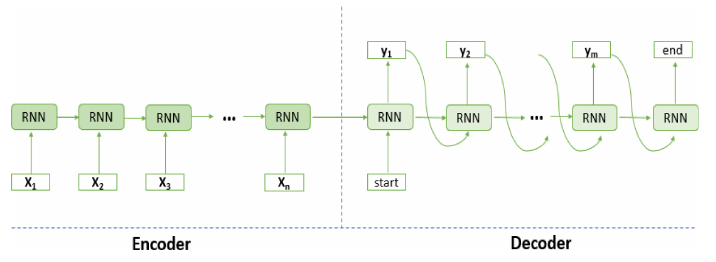
\includegraphics[height=6cm]{encoder_decoder.png}
	\end{center}
	\caption{معماری پایه‌‌ی مدل کدگذار-کدگشا \cite{RL_survey}}
	\label{fig:encoder_decoder}
	\medskip
	\small
\end{figure}

یائو\LTRfootnote{Yao}
و همکاران مدل کدگذاری دوگانه را برای خلاصه‌سازی انتزاعی پیشنهاد داده‌اند. این مدل برای درک بهتر روابط بین متن ورودی و خلاصه مرجع بازنمایی متن ورودی و بازنمایی خلاصه‌ی مرجع را می‌آموزد. همانطور که در شکل \ref{fig:dual_encoder} نشان داده شده است.
%کدگذاری دوگانه به مدل اجازه می‌دهد تا دو نمایش متفاوت از متن را بیاموزد: نمایش متن ورودی و نمایش خلاصه مرجع. این به مدل اجازه می‌دهد تا روابط بین متن ورودی و خلاصه مرجع را بهتر درک کند، که می‌تواند منجر به خلاصه‌های دقیق‌ و حاوی اطلاعات مفید شود.
این مدل از یک کدگذار اولیه، یک کدگذار ثانویه و یک کدگشا مجهز به مکانیزم توجه تشکیل شده است و هر سه ماژول فوق از واحد بازگشتی دروازه‌ای
\LTRfootnote{gated recurrent unit (GRU)}
استفاده می‌کنند. 
کدگذار اولیه بردارهای معنایی هر کلمه در ترتیب ورودی را محاسبه می‌کند. کدگذار ثانویه وزن اهمیت هر کلمه در ترتیب ورودی و بردارهای معنایی مربوطه را دوباره محاسبه می‌کند. در نهایت کدگشا با مکانیسم توجه به صورت مرحله‌ای کدگشایی می‌کند و در هر مرحله یک توالی خروجی با طول ثابت جزئی ایجاد می‌کند. در این مدل کدگذار ثانویه عملیات کدگذاری را براساس ورودی هر مرحله و خروجی مرحله‌ی قبل انجام می‌دهد بنابراین کیفیت متون قبلی تولید شده توسط کدگشا بر خروجی‌های جدید تاثیر می‌گذارد
 \cite{yao2018dual}.



\begin{figure}[!h]
	\begin{center}
		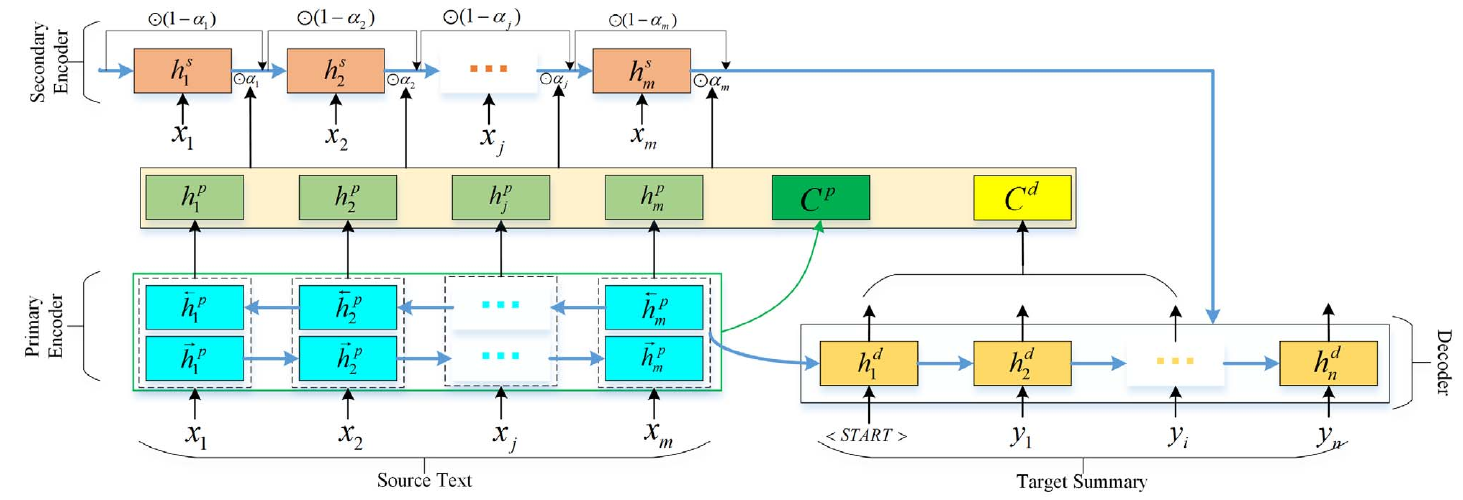
\includegraphics[height=5cm]{dualـencoder.png}
	\end{center}
	\caption{معماری پایه‌‌ی مدل دوگانه‌ی کدگذار 	 \cite{yao2018dual}}
	\label{fig:dual_encoder}
	\medskip
	\small
\end{figure}


مدل کدگذاری دوگانه مدل سلسله مراتبی متغیر بر اساس مدل کدگذاری دوگانه برای خلاصه‌سازی متقاطع زبانی\LTRfootnote{cross-lingual}
پیشنهاد شده است. این مدل شامل دو متغیر نهفته محلی و یک متغیر نهفته جامع است. از متغیرهای نهفته محلی برای بازسازی ترجمه و خلاصه زبان مبدأ و از متغیر نهفته سراسری برای تولید خلاصه بین زبانی استفاده می‌شود. قسمت کد گذار این مدل دو بخش دارد که هر بخش وظیفه‌ی تولید یکی از متغیرهای نهفته محلی را دارد و بخش کدگشا با استفاده از نمایش‌های نهفته‌ی محلی خلاصه‌ی نهایی را تولید می‌کند.
ساختار سلسله مراتبی این مدل به آن اجازه می‌دهد تا رابطه سلسله مراتبی بین ترجمه، خلاصه‌سازی و خلاصه‌سازی بین زبانی را بیاموزد \cite{variational}.

\begin{figure}[!h]
	\begin{center}
		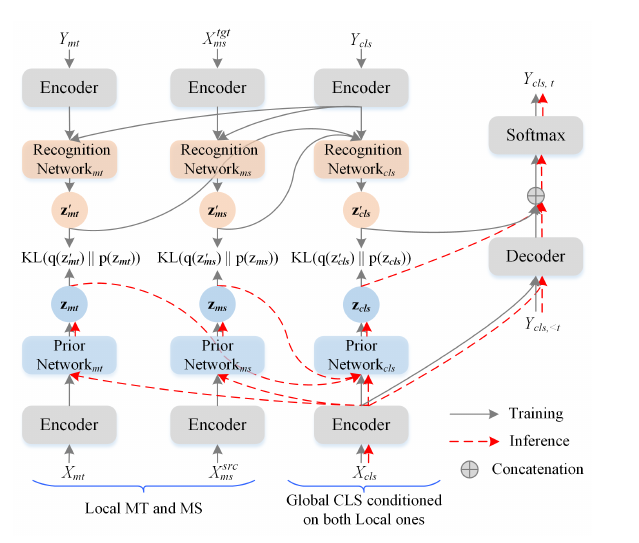
\includegraphics[height=12cm]{Variational Hierarchical Model.png}
	\end{center}
	\caption{معماری پایه‌‌ی مدل سلسله مراتبی متغیر برای خلاصه‌سازی متقابل زبانی \cite{variational}}
	\label{fig:vahie_model}
	\medskip
	\small{
		متغیرهای محلی $ z_mt $ و $ z_ms $ به ترتیب برای ترجمه و خلاصه‌سازی و متغیر جامع $ z_cls $ برای خلاصه‌سازی بین زبانی طراحی شده‌اند. خطوط خاکستری نشان‌دهنده فرآیند آموزشی است که مسئول تولید
		($ z' _{mt} $، $ z'_{ms} $، $ z'_{cls} $)
		از توزیع پسین متناظر پیش‌بینی‌شده توسط شبکه‌ است. خطوط قرمز خط چین نشان دهنده فرآیند استنتاج برای تولید نمایش‌‌های نهفته
		($ z _{mt} $، $ z_{ms} $، $ z_{cls} $)
		از توزیع‌های پیش بینی شده توسط شبکه‌های قبلی است. }
\end{figure}



%\subsection{روش‌های ارايه شده برای متون کوتاه }


%\subsection{روش‌های ارايه شده برای متون طولانی }


\section{روش‌های مبتنی بر مدل ترنسفورمر‌}
با ظهور ترنسفورمرها\LTRfootnote{transformers}
، بهبودهای قابل توجهی در کیفیت نتایج خلاصه‌سازی خودکار به وجود آمد. ترنسفومرها با استفاده از مکانیزم توجه به خود\LTRfootnote{Self-attention}
شباهت بین ورودی‌ها را بدون توجه به موقعیت موازی آن‌ها با حضور مستقل هر توکن در توالی ورودی مدل می‌کنند و به طور مؤثر مشکلات شبکه‌های بازگشتی را حل می‌کنند \cite{vaswani2017attention}. یکی از جهت‌گیری‌های رایج پژوهشی، اصلاح یا تطبیق ترنسفورمرها و مدل‌های زبانی از پیش آموزش دیده با وظایف مختلف مانند خلاصه‌سازی است. مدل‌های مبتنی بر مدل‌های زبانی از پیش آموزش دیده که با هدف خلاصه‌سازی انتزاعی طراحی شده‌اند از ویژگی‌های معنایی و متنی غنی بازنمایی‌های زبان برای بهبود کیفیت و دقت خلاصه‌‌ها استفاده می‌کنند.



پان
\LTRfootnote{Pan}
و همکاران یک مدل خلاصه‌سازی بر اساس مدل برت را پیشنهاد کرده‌اند. نویسندگان استدلال می‌کنند که خلاصه‌های تولید شده توسط مدل‌های خلاصه‌سازی متن موجود که موضوع متن را در نظر نمی‌گیرند، مرتبط یا حاوی اطلاعات مفید نیستند. 
مدل ارائه شده که تی‌برت‌سام\LTRfootnote{T-BERTSum}
نامیده می‌شود از سه بخش ایجاد بازنمایی، مدل موضوعی عصبی\LTRfootnote{Neural Topic Model(NTM)}
و مدل خلاصه‌سازی تشکیل شده است. ساختار مدل را در شکل \ref{fig:tBert_model} نشان داده شده است.
\begin{figure}[!h]
	\begin{center}
		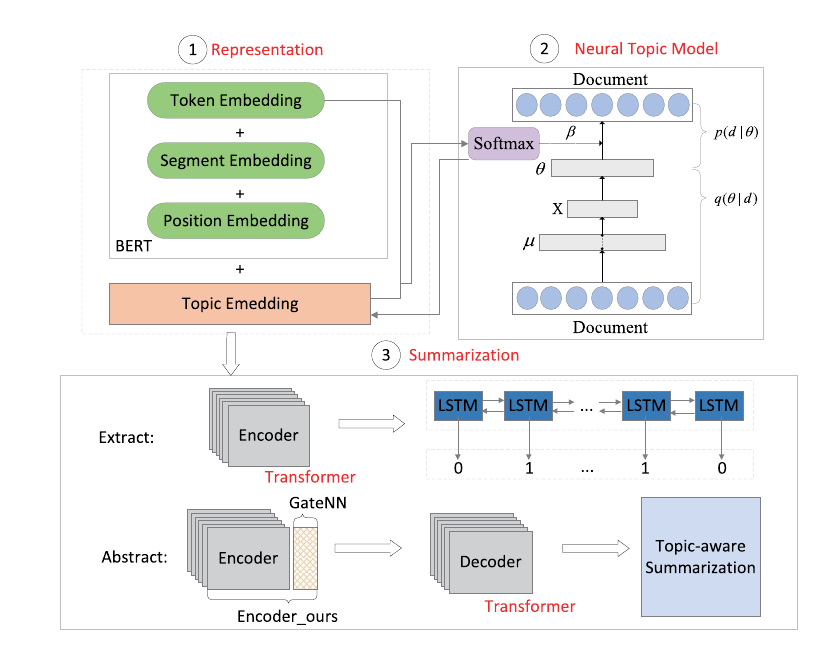
\includegraphics[height=10cm]{tbertsum_framework.png}
	\end{center}
	\caption{معماری مدل تی‌برت‌سام \cite{Ma2022TBERTSumTT}}
	\label{fig:tBert_model}
	\medskip
	\small
\end{figure}



همانطور که در شکل \ref{fig:tBert_embded} نشان داده شده است، بازنمایی ایجاد شده برای هر جمله ورودی، با استفاده از یک شبکه‌ی ترنسفورمر دوسویه‌ی\LTRfootnote{bidirectional}
چند لایه و حاصل جمع چهار نوع تعبیه ( تعبیه نشانه\LTRfootnote{token embedding}
، تعبیه قطعه\LTRfootnote{segment embedding}
، تعبیه موقعیت و تعبیه موضوع) به دست ‌می‌آید که تعبیه موضوع در این مقاله معرفی شده و سه تعبیه دیگر مشابه مدل برت هستند. وجود تعبیه موضوع در تولید بازنمایی هر کلمه یا جمله موجب افزودن اطلاعات پیش زمینه‌ای به هر کلمه و حل مشکل چند معنایی می‌شود.
\begin{figure}[!h]
	\begin{center}
		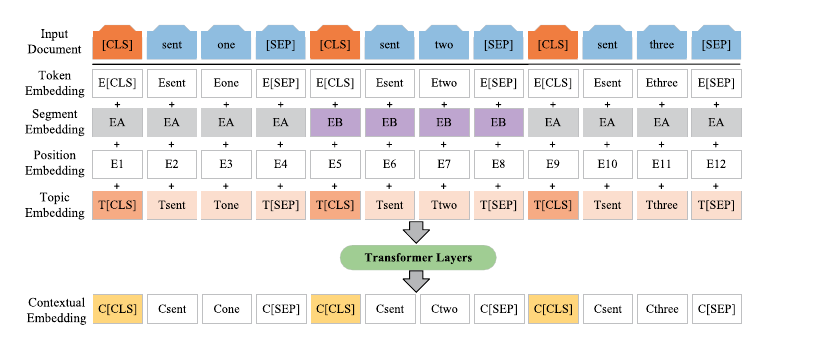
\includegraphics[height=7cm]{TbertSum_embedding.png}
	\end{center}
	\caption{ تعبیه مدل تی‌برت‌سام \cite{Ma2022TBERTSumTT}}
	\label{fig:tBert_embded}
	\medskip
	\small
\end{figure}

مدل موضوعی عصبی وظیفه‌ی ایجاد تعبیه موضوعی را دارد. این مدل دارای دو جزء است: یک شبکه مولد و یک شبکه استنتاج.
شبکه مولد یک سند را به عنوان ورودی می‌گیرد و یک توزیع موضوعی را بر روی کلمات موجود در سند خروجی می‌دهد.
%\todo{مفهوم درست نیست}
شبکه استنتاج یک سند را به عنوان ورودی می‌گیرد و خروجی آن پارامترهای توزیع موضوع است. 
بخش خلاصه‌سازی مدل مبتنی بر معماری کدگذار - کدگشای ترنسفورمر است. کدگذار بازنمایی ایجاد شده را به عنوان ورودی می‌گیرد و دنباله‌ای از حالت‌های پنهان را تولید می‌کند. سپس کدگشا با استفاده از  حالت‌های پنهان و متن خلاصه را تولید می‌کند. همانطور که در شکل 
\ref{fig:tBert_transformer}
نشان داده شده است، به منظور فیلتر کردن اطلاعات کلیدی توالی ورودی، شبکه دروازه‌ای قبل از کدگشا اضافه می‌شود.
این شبکه برای کنترل جریان اطلاعات از دنباله ورودی به دنباله خروجی افزوده شده است و باعث می‌شود کدگشا بر روی تولید خلاصه از اطلاعات کلیدی و حذف اطلاعات غیرضروری تمرکز کند. این مدل می‌تواند خلاصه‌هایی تولید کند که مرتبط با موضوع متن و حاوی اطلاعات مفید باشد و قابلیت تطبیق با حوزه‌های مختلف را دارد.
%\todo{جمله‌ی اخر تکراری هست}

\begin{figure}[!h]
	\begin{center}
		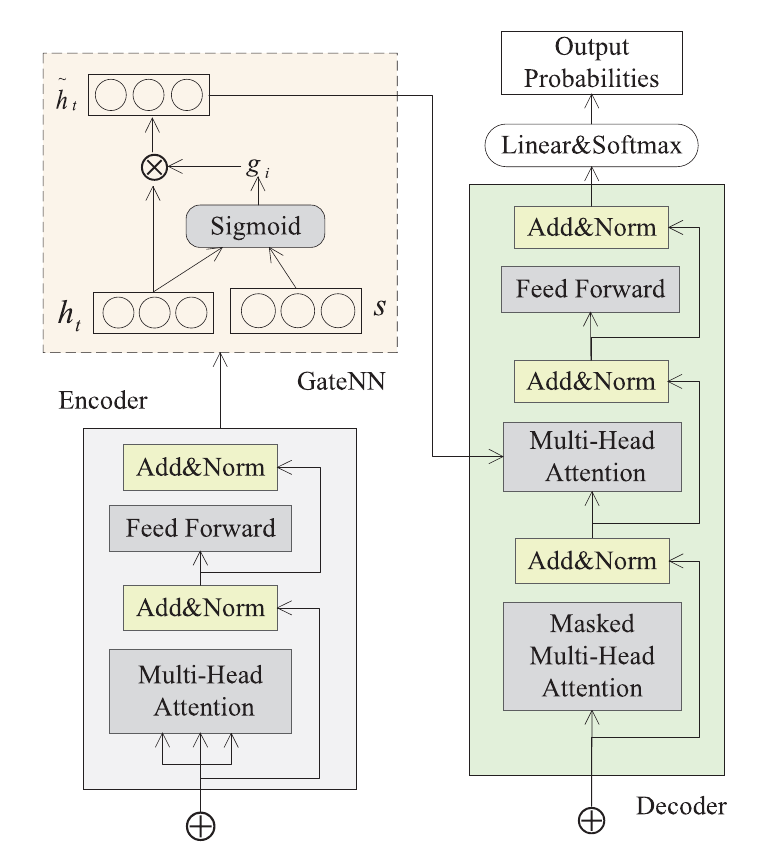
\includegraphics[height=10cm]{tbertsum_transformer.png}
	\end{center}
	\caption{ معماری ترنسفورمر تی‌برت‌سام \cite{Ma2022TBERTSumTT}}
	\label{fig:tBert_transformer}
	\medskip
	\small
	\centerline{	این مدل شامل شبکه‌ی دروازه‌ای و کدگذار-کدگشا با توجه چند سر می‌باشد \cite{Ma2022TBERTSumTT}}
	
\end{figure}
%\todo{ادیت}

اکثر مدل‌های خلاصه‌سازی انتزاعی موجود برای تولید خلاصه‌های با طول ثابت طراحی شده‌اند، بنابراین سو
\LTRfootnote{Ming-Hsiang Su}
و همکاران یک مدل دو مرحله‌ای مبتنی بر تنرسفورمر ارائه دادند که خلاصه‌های انتزاعی با طول متغیر را با توجه به تقاضای کاربر تولید کند. مطابق شکل  \ref{fig:two_stage_model}مدل پیشنهادی با تقسیم متن ورودی به بخش‌ها ، استخراج اطلاعات کلیدی و تولید خلاصه‌ی هر بخش، خلاصه‌ی انتزاعی با طول متغیر تولید می‌کند \cite{twostage}. بخش‌‌های مدل ارائه شده به شرح زیر است.
\begin{itemize}
	\item {
		بخش‌بندی متن: این مرحله متن ورودی را به تعدادی قسمت از پیش تعیین شده تقسیم می‌کند. تعداد بخش‌ها را می‌تواند توسط کاربر مشخص شود یا با توجه به نسبت دلخواه طول ورودی تنظیم کرد.
		برای شناسایی مرزهای بین بخش‌ها از مدل $ BERT-biLSTM $ استفاده می‌شود. این مرحله تضمین می‌کند که مرحله خلاصه‌سازی انتزاعی بر روی بخش‌های منسجم متن انجام می‌شود. هدف این بخش یافتن نقاط تقسیم‌بندی است که نشان دهنده تغییر موضوع در متن است و  به بهبود کیفیت خلاصه‌های تولید شده کمک می‌کند. 
	}
	\item {
		خلاصه‌سازی استخراجی: پس از تقسیم‌بندی متن، با استفاده از یک مدل خلاصه‌سازی استخراجی مبتنی بر برت‌سام
		\LTRfootnote{BertSum}
		مهم‌ترین جمله را از هر بخش استخراج می‌شود.
	}
	\item {
	خلاصه‌سازی اسناد: با استفاده از جملات استخراج شده این ماژول خلاصه سرفصل سند ورودی را تولید می‌کند که این خلاصه  به عنوان خروجی هدف در مرحله آموزش مدل دو مرحله‌ای استفاده می‌شود. مدل ترنسفورمر سند به حل مشکل تغییر طول ورودی و خروجی در کار خلاصه‌سازی کمک می‌کند.
	}
	\item{
	خلاصه‌سازی بخش: این ماژول وظیفه‌ی تولید خلاصه برای بخش‌های به دست آمده از مرحله تقسیم‌بندی متن را دارد.
}
\item{
آموزش مشارکتی:  برای آموزش متناوب ماژول خلاصه‌سازی بخش و ماژول خلاصه‌سازی اسناد تا زمان همگرایی آموزش مشارکتی اعمال می‌شود. این فرآیند به بهینه سازی عملکرد هر دو ماژول کمک می‌کند.}
\item{
	ایجاد خلاصه با طول متغیر:پس از اینکه متن ورودی به بخش‌های مختلف تقسیم شد، هر بخش از ماژول خلاصه‌سازی بخش عبور می‌کند تا یک خلاصه انتزاعی مبتنی بر جمله ایجاد کند. سپس این خلاصه‌های مبتنی بر جمله به هم متصل می‌شوند تا خلاصه انتزاعی با طول متغیر را تشکیل دهند. این فرآیند الحاق تضمین می‌کند که خلاصه تولید شده شامل اطلاعات تمام بخش های متن ورودی است.}
	
\end{itemize}
با ترکیب روش‌های استخراجی و انتزاعی در مدل خلاصه‌سازی دو مرحله‌ای، رویکرد پیشنهادی می‌تواند خلاصه‌های انتزاعی روان و با طول متغیر را با توجه به خواسته‌های کاربر تولید کند \cite{twostage}.




%خلاصه‌سازی اسناد: در مرحله دوم از جملات استخراج شده برای آموزش ماژول خلاصه‌سازی اسناد استفاده می‌شود. این ماژول یک خلاصه سرفصل از کل ورودی متن ایجاد می‌کند. پارامترهای این ماژول با در نظر گرفتن امتیازات ضرر ماژول خلاصه‌سازی اسناد و ماژول خلاصه‌سازی بخش به روز می‌شود.

%خلاصه‌سازی بخش‌ها: بخش‌های به دست آمده از مرحله تقسیم‌بندی متن برای آموزش ماژول خلاصه‌سازی در مرحله اول استفاده می‌شود. این ماژول یک خلاصه بر اساس جمله برای هر بخش تولید می‌کند. امتیازات ضرر ماژول خلاصه‌سازی سند و ماژول خلاصه‌سازی بخش برای به روز رسانی پارامترهای ماژول خلاصه‌سازی بخش در نظر گرفته می‌شود.



%خلاصه‌سازی با طول متغیر: در طول آزمایش، خروجی‌های ماژول خلاصه‌سازی بخش به هم متصل می‌شوند تا نتیجه خلاصه‌سازی انتزاعی با طول متغیر ارائه شود. تعداد بخش‌ها را می‌توان توسط کاربر مشخص کرد یا با توجه به نسبت دلخواه طول ورودی تنظیم کرد.

%با ترکیب روش‌های استخراجی و انتزاعی در مدل خلاصه‌سازی دو مرحله‌ای، رویکرد پیشنهادی می‌تواند خلاصه‌های انتزاعی روان و با طول متغیر را با توجه به خواسته‌های کاربر تولید کند \cite{twostage}.
%\todo{ ادیتش کن}
%این مدل می‌تواند خلاصه‌های انتزاعی با طول متغیر را با توجه به خواسته‌های کاربر ایجاد کند. این یک پیشرفت نسبت به مدل‌های قبلی است زیرا می‌تواند به طور همزمان به خلاصه‌سازی انتزاعی روان و با طول متغیر دست یابد.

\begin{figure}[!h]
	\begin{center}
		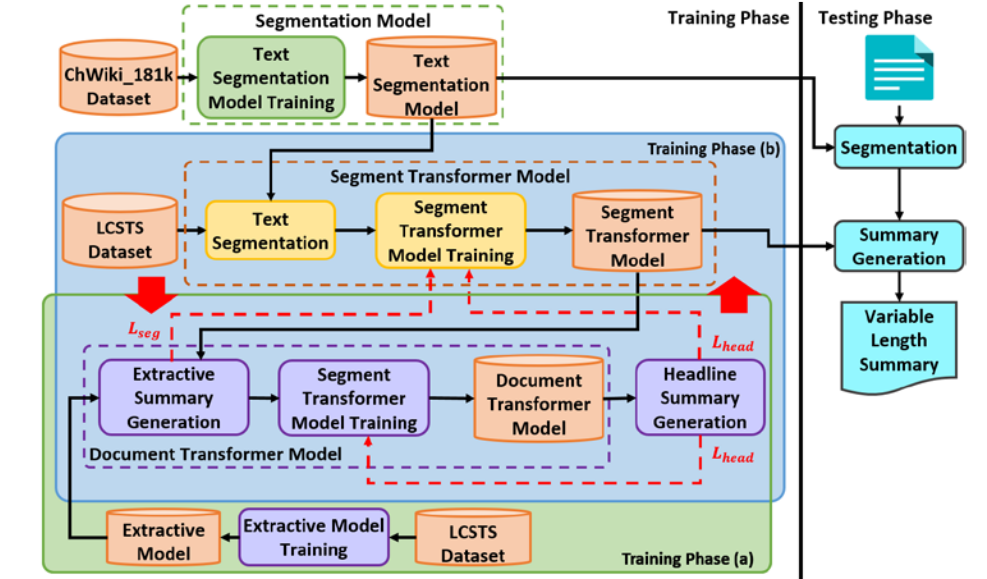
\includegraphics[height=10cm]{two-stage model.png}
	\end{center}
	\caption{ چهارچوب ایجاد خلاصه با طول متغیر \cite{twostage}}
	\label{fig:two_stage_model}
	\medskip
	\small	
\end{figure}




لوئيس و همكاران مدلي با نام بارت 
\LTRfootnote{BART}
ارائه دادند. اين مدل مشابه با مدل اصلي ترنسفورمر، ساختاري كدگذار-کدگشا دارد. بر خلاف سادگي، به دليل داشتن كدگذار دو طرفه و كدگشاي چپ به راست اين مدل را مي‌توان نسخه عمومي‌تري از برت و جي‌پي‌تي 
\LTRfootnote{GPT}
 دانست. بارت در عمليات توليد متن، مانند ترجمه ماشيني يا خالصه‌سازي انتزاعي متن، و همچنين در فهم متن كاربرد دارد و با استفاده از اهداف کدگذاری خودکار حذف نویز آموزش می‌بیند. برای پیش‌آموزش بارت نواقصی در سندهای ورودی ایجاد می‌شود و با بهینه کردن تابع زیان آنتروپی-متقاطع \LTRfootnote{‫‪cross-entropy‬‬}
  بین خروجی‌های کدگشا و سند اولیه، متن بازسازی می‌شود. همانطور که در شکل\ref{fig:bart} نشان داده شده است این مدل طیف گسترده‌ای از نویز ‌ها از جمله پوشاندن توکن، حذف توکن، پر کردن متن، چرخش سند، به هم ریختن جمله (به هم زدن تصادفی ترتیب کلمه یک جمله) را استفاده  می‌کند \cite{lewis-etal-2020-bart}. 
%\todo{یک کم دیگه اضافه کن}
\begin{figure}[!h]
	\begin{center}
		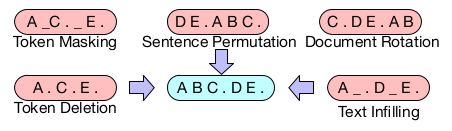
\includegraphics[height=4cm]{bart2.png}
	\end{center}
	\caption{ عمل‌های پیش‌آموزش بارت \cite{lewis-etal-2020-bart}}
	\label{fig:bart}
	\medskip
	\small
	%ورودی‌های کدگذار نیازی به هم‌سویی با خروجی‌های کدگشا ندارند، که امکان تبدیل نویز دلخواه را فراهم می‌کند. در اینجا، یک سند با جایگزین کردن دهانه‌های متن با نمادهای ماسک خراب شده است. سند خراب (سمت چپ) با یک مدل دو طرفه کدگذاری می‌شود و سپس احتمال سند اصلی (سمت راست) با کدگشای خودبازگشتی محاسبه می‌شود. برای تنظیم دقیق، یک سند خراب به رمزگذار و رمزگشا وارد می‌شود و ما از نمایش‌هایی از حالت پنهان‌ نهایی کدگشا استفاده می‌کنیم \cite{lewis-etal-2020-bart}.
\end{figure}


با اين كه بارت دقت خلاصه‌سازی انتزاعي متن را بهبود بخشيد، ولي مراحل پيش‌آموزش آن، مختص خلاصه‌سازی انتزاعي متن نیستند، در نتیجه در سال 2020 مدلي تحت عنوان پگاسوس\LTRfootnote{PEGASUS}
توسط ژنگ و همكاران ارائه شد كه معماري مشابه با بارت داشت ولي پيش‌آموزش آن مختص خلاصه‌سازی انتزاعي متن بود.
مدل پگاسوس
یک مدل دنباله به دنباله کدگذار کدگشا مبتنی بر ترنسفورمر است که بر روی مجموعه‌های متنی بدون نظارت با هدف تولید جملات فاصله‌افتاده\LTRfootnote{‫‪gap‬‬ ‫‪sentences‬‬ ‫‪generation‬‬}
از قبل آموزش داده شده است \cite{zhang2020pegasus}.

این مدل دو روش پيش‌آموزش را معرفي كرده است كه در ادامه به شرح آنها مي‌پردازيم:
\begin{enumerate}
	\item {
		توليد جملات فاصله‌افتاده : فرضی مطرح شده است كه اگر عمل پيش‌آموزش مدل به وظایف
		پايين‌دست\LTRfootnote{downstream task}
		نزديك‌تر باشد، نتیجه نهايي بهتر و همچنين تنظیم دقیق پارامترها
		\LTRfootnote{fine-tuning}
		سريع‌تر خواهد بود. با توجه به اين كه اين مدل قرار است فقط براي خلاصه‌سازی انتزاعي متن استفاده شود، عمل
		پيش‌آموزش مشابه توليد متن‌هاي خلاصه از يك سند ورودي تعریف شده‌است. تعدادي از جملات انتخاب شده و هر جمله
		به طور كامل با توكن $ [MASK1] $ جايگزين ميشود. براي انتخاب اين جملات، سه راه پيشنهاد
		شده است.
		\begin{itemize}
			\item {
				انتخاب تصادفي: $ m $جمله به صورت تصادفي از متن انتخاب شده و پنهان مي‌شوند.
			}
			\item{
				انتخاب جملات اول متن: $ m $جمله اول متن پنهان مي‌شوند زیرا اغلب جملات ابتداي متن نسبت به جملات بعدی مهم‌ترهستند.
			}
			\item{
				انتخاب جملات مهم متن: براي انتخاب $ m $ جمله مهم متن از تقريب معيار ارزيابي روژ-۱
				استفاده می‌شود. به ازای هر
				جمله از متن، يك دوتايي از آن جمله و متن سند فاقد آن جمله ساخته شده و ارزيابي
				مي‌شود كه چقدر ممکن است اين جمله، خلاصه سند فاقد آن جمله باشد. جملاتي
				كه امتیاز بالاتر گرفته‌اند از نظر خلاصه بودن مهم‌تر هستند و پنهان می‌شوند.
			}
			
			
		\end{itemize}
	}
	\item{
		 مدل زباني پوشيده شده: مشابه مدل برت ۵۱ درصد از توكن‌هاي متن ورودي انتخاب
		مي‌شوند و سپس 80 درصد از اين توكن‌ها، با توكن $ [MASK2] $ و10 درصد توكن‌ها با يك توكن
		تصادفي جايگزين می‌شوند. 10 درصد ديگر بدون تغيير باقي می‌ماند.
		شكل \ref{fig:pegasus} اعمال همزمان اين دو عمل، يعني توليد جمالت فاصله افتاده و مدل زباني پوشيده شده
		را بر روي يك ورودی نشان می‌دهد.
	}
\end{enumerate}

\begin{figure}[!h]
	\begin{center}
		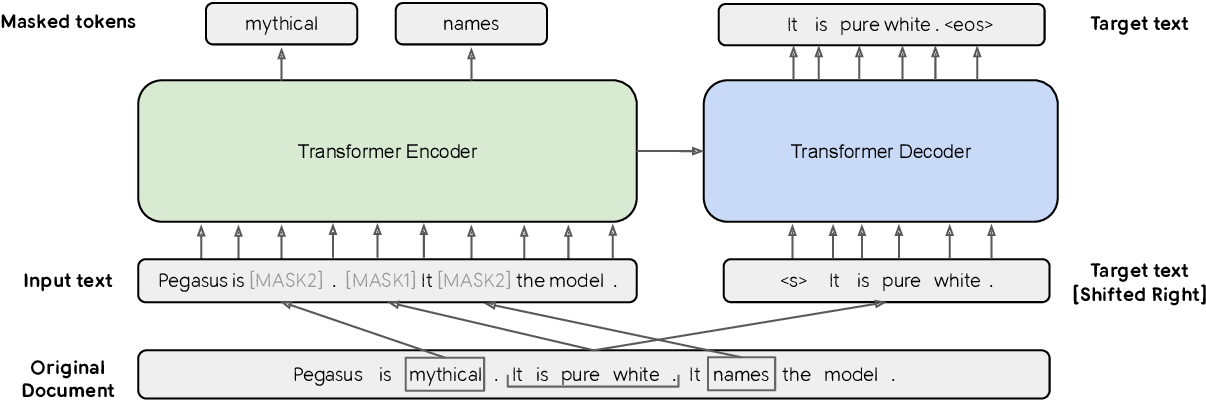
\includegraphics[height=5cm]{pegasus.png}
	\end{center}
	\caption{ ساختار مدل پگاسوس \cite{zhang2020pegasus}}
	\label{fig:pegasus}
	\medskip
	\small{
		معماری پایه پگاسوس یک کدگذار-کدگشا ترنسفورمر استاندارد است. جملات فاصله‌افتاده و مدل زبانی پوشیده شده به طور همزمان در این مثال به عنوان اهداف پيش‌آموزش اعمال می‌شوند. در اصل سه جمله وجود دارد. یک جمله با $ [MASK1] $ پوشانده شده و به عنوان متن تولید هدف جملات فاصله‌افتاده استفاده می‌شود. دو جمله دیگر در ورودی باقی می‌مانند و برخی از نشانه‌ها به طور تصادفی توسط$ [MASK2] $پوشانده می‌شوند
		 \cite{zhang2020pegasus}.}
\end{figure}

کدیا
\LTRfootnote{Kedia}
و همکاران الگوریتم حداکثرسازی نقطه-محصول فرایادگیری (ام‌دات)\LTRfootnote{Meta-Learned Dot-Product Maximization (MDot)}
را برای بهبود پگاسوس پیشنهاد دادند. این الگوریتم بر اساس ایده به حداکثر رساندن حاصل‌ضرب نقطه‌ای بین گرادیان‌های مدل در نقاط مختلف آموزش با استفاده از تکنیکی به نام تفاوت‌های محدود\LTRfootnote{finite differences}
است. این الگوریتم از نظر محاسباتی کارآمد است و می‌تواند برای مدل‌های بزرگ مانند برت اعمال شود و سربار محاسباتی را کاهش بدهد \cite{sherborne2023meta}.
عملکرد مناسب مدل پگاسوس در خلاصه‌سازی متون باعث شده بهترین مدل خلاصه‌سازی متون کوتاه مبتنی بر مدل پگاسوس و تکنیک تنظیم\LTRfootnote{regularization}
ام‌دات باشد.

\begin{figure}[!h]
	\begin{center}
		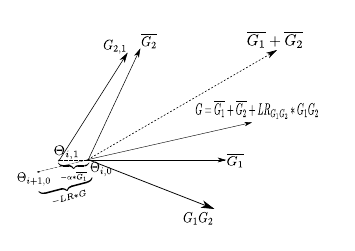
\includegraphics[height=6cm]{Mdot.png}
	\end{center}
	\caption{ الگوریتم ام‌دات \cite{sherborne2023meta}}
	\label{fig:Mdot}
	\medskip
	\small{
		محاسبه گرادیان برای به حداکثر رساندن محصول نقطه‌ای با استفاده از تقریب تفاضل محدود و استفاده از آن برای تنظیم گرادیان استاندارد \cite{sherborne2023meta}.
	}
\end{figure}


%\section{روش‌های مبتنی بر مدل‌های از پیش آموزش دیده}



\subsection{ایده‌های ارائه شده بهبود خلاصه‌سازی متون طولانی }


یکی از مشکلات مدل ترنسفومر در خلاصه‌سازی متون طولانی، حافظه‌ی درجه دوم، پیچیدگی‌های محاسباتی و تعداد زیاد عملیات می‌باشد. برای حل این چالش‌ها ایده‌های مختلفی ارائه شده است. به عنوان مثال شبکه‌ی ریفورمر\LTRfootnote{‫‪Reformer‬‬}
برای حل چالش‌های محاسباتی مرتبط با پردازش دنباله‌های طولانی متن ارائه شده است. لایه‌های برگشت‌پذیر\LTRfootnote{reversible layers}
معرفی شده در این مقاله امکان بازسازی ورودی از خروجی را در طول گذر به عقب را فراهم می‌کنند که موجب  کاهش نیازهای حافظه و امکان پردازش کارآمد دنباله‌های طولانی  می‌شود.
علاوه بر این، ریفورمر از تکه تکه کردن برای پردازش بخش‌های کوچک‌تر ورودی به طور مستقل استفاده می‌کند که موازی‌سازی را ممکن می‌کند و مصرف حافظه را کاهش می‌دهد. همچنین استفاده از درهم‌سازی حساس به مکان\LTRfootnote{‫‪locality-sensitive‬‬ ‫‪hashing‬‬ ‪(LSH‬)} 
 در مکانیسم توجه منجر به محاسبه توجه کارآمدتر می‌شود. درهم‌سازی حساس به مکان با توجه به زیرمجموعه‌ای از نشانه‌ها بر اساس مقادیر هش آنها، محاسبه توجه کامل را تقریب می‌زند. علاوه بر این، ریفورمر از کدگذاری‌های موقعیت محوری برای کدگذاری اطلاعات موقعیت توکن‌ها به صورت فشرده استفاده می‌کند. این تکنیک‌ها مجموعاً مدل ریفورمر را  مقیاس‌پذیر می‌سازد، و آن را قادر می‌سازد تا دنباله‌های طولانی متن را مدیریت کند و در عین حال عملکرد رقابتی را در وظایف مختلف پردازش زبان طبیعی حفظ کند \cite{reformer}.
%\todo{ادیت}

 شبکه‌ی ترنسفورمر پراکنده\LTRfootnote{sparse }
با معرفی فاکتورسازی‌ ماتریس پراکنده‌ی توجه، زمان و حافظه مورد نیاز را به کاهش می‌دهد.
با استفاده از پراکندگی، مدل می‌تواند تنها به زیرمجموعه‌ای از نشانه‌های ورودی توجه کند و روی مرتبط‌ترین اطلاعات تمرکز کند و بقیه را نادیده بگیرد. این رویکرد پیچیدگی محاسباتی را کاهش می‌دهد و مدل می‌تواند توالی‌های طولانی‌ را مدیریت کند \cite{child2019generating}.
 مشابه شبکه‌ی ترنسفورمر پراکنده مدل بیگ‌برد که\LTRfootnote{‫‪Big‬‬ ‫‪Bird‬‬}
با استفاده از مکانیزم توجه پراکنده\LTRfootnote{‫‪Sparse‬‬ ‫‪attention‬‬}
 عملکرد ترنسفورمر را در مواجه با دنباله‌ی کلمات
%\LTRfootnote{‫‪sequence‬‬}
طولانی بهبود می‌بخشد، نوآوری‌های دیگری مانند توجه جامع\LTRfootnote{global attention}
را معرفی می‌کند. در این مدل توکن‌های خاص به تمام توکن‌های دیگر در دنباله توجه می‌کنند و وابستگی‌های دوربرد را بهتر از سایر روش‌ها به دست می‌آورند. همچنین  فرآیند پالایش تکراری  وزن‌های توجه را برای بهبود عملکرد مدل اصلاح می‌کند \cite{zaheer2020big}. 
%\todo{ادیت}


%ژیائو و کارنی \LTRfootnote{‫Xiao \& ‬‬ ‫‪Carenini‬‬} با تمرکز برکاهش تکرار و افزونگی در خلاصه‌سازی اسناد طولانی مدلی طراحی کرده‌اند که کدگشایی آن براساس مکانیزم توجه آگاه از افزونگی می‌باشد. علاوه بر این تابع ضرر \LTRfootnote{‫‪Loss‬‬ ‫‪function‬‬} طراحی کرده‌اند که برای تعادل بین اهمیت و افزونگی مناسب باشد. این روش باعث انتخاب جملات مهم و غیر زائد می‌شود \todo{دوباره بنویس} \cite{xiao2020systematically}

در سال‌های اخیر ایده‌های مختلفی برای بهبود کیفیت خروجی مدل خلاصه‌سازی خودکار اسناد بلند ارائه شده است. به عنوان مثال پایل\LTRfootnote{‫‪Pilault‬‬}
و همکاران که برای بهبود خلاصه انتزاعی نهایی متون طولانی از رویکرد ترکیبی استخراجی-انتزاعی با استفاده از مدل زبانی از پیش آموزش دیده جی‌پی‌تی-دو\LTRfootnote{GPT-2}
استفاده می‌کنند. در این مدل مرحله استخراج ساده قبل از تولید خلاصه انجام می‌شود، سپس برای شرطی کردن مدل زبانی ترنسفورمر بر روی اطلاعات مربوط قبل از تولید خلاصه استفاده می‌شود. این رویکرد در مقایسه با کارهای قبلی که از مکانیزم کپی استفاده می‌کنند، خلاصه‌های انتزاعی بیشتری تولید می‌کند \cite{pilault2020extractive}. 
پانگ\LTRfootnote{Pang}
و همکاران یک ساختار سلسله مراتبی برای اسناد طولانی فرض کرده‌اند. در این ساختار سطح بالا بر وابستگی دوربرد تمرکز می‌کند و سطح پایین جزئیات را حفظ می‌کند. 
در استنتاج از پایین به بالا، تعبیه‌های متنی نشانه‌ها با استفاده از توجه محلی محاسبه می‌شوند و برای دریافت وابستگی‌های دوربرد و زمینه جامع، استنتاج از بالا به پایین برای نمایش‌های توکن اعمال می‌شود. یک ساختار پنهان چند مقیاسی دو سطحی استفاده می‌شود، که در آن سطح پایین شامل نمایش‌های نشانه‌ای است که توسط استنتاج پایین به بالا محاسبه می‌شود، سپس با اعمال مکانیزم توجه به سطوح بزرگ‌تر روابط بین بخش‌های مختلف سند را بدست می‌آورد. ساختار مدل را در شکل \ref{fig:top_down} نشان داده شده است. روش پیشنهادی یک رویکرد جدید امیدوارکننده برای خلاصه‌سازی اسناد طولانی است و نسبت به روش‌های قبلی کارآمدتر و موثرتر است \cite{pang2023long}.
% این چارچوب استنتاج از پایین به بالا را با استنتاج از بالا به پایین برای بهبود استنتاج نمایش توکن هم‌افزایی می‌کند 

\begin{figure}[!h]
	\begin{center}
		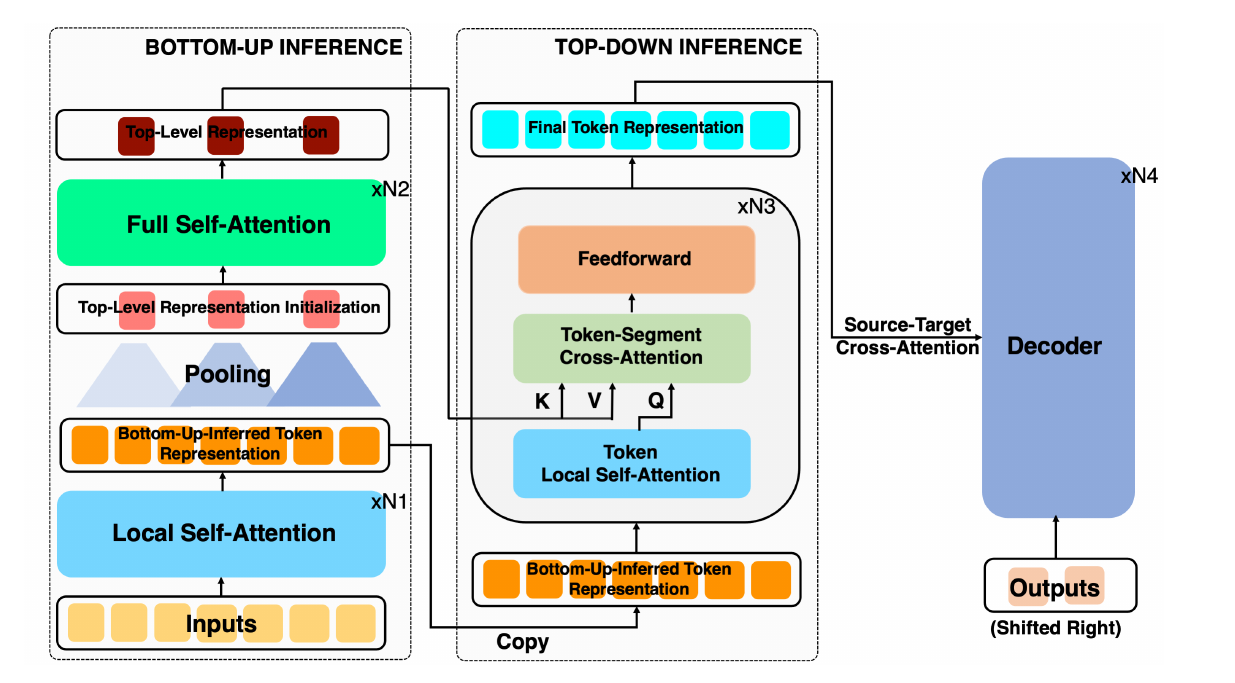
\includegraphics[height=8cm]{top_down.png}
	\end{center}
	\caption{ معماری مدل ترنسفورمر از بالا به پایین \cite{pang2023long}}
	\label{fig:top_down}
	\medskip
	
\end{figure}


%. روش پیشنهادی یک رویکرد جدید امیدوارکننده برای خلاصه‌سازی اسناد طولانی است و بهترین عملکرد در خلاصه‌سازی متون طولانی را دارد
%\todo{ادیت}

جیدیوتیس و همکاران شیوه‌ی تقسیم و غلبه ( دنسر)\LTRfootnote{Divide-and-ConquER (DANCER)}
را برای بهبود خلاصه‌سازی اسناد طولانی پیشنهاد کرده اند.این روش به طور خودکار خلاصه یک سند را به چند بخش‌ تقسیم می‌کند و هر یک از این بخش‌ها را به بخش مناسب سند جفت می‌کند تا خلاصه‌های هدف متمایز ایجاد کند. شیوه‌ی معرفی شده در نظر می‌گیرد که متون طولانی به صورت بخش‌های گسسته ساختاربندی شده‌اند. 

برای مطابقت هر قسمت از خلاصه با بخشی از سند در دنسر از معیار روژ\LTRfootnote{ROUGE}
استفاده ‌می‌شود. در این روش معیار روژ-ال بین هر یک از جملات خلاصه و تمام جملات سند محاسبه می‌شود و هر جمله‌ی خلاصه هدف به بخش حاوی جمله با بیشترین روژ- ال نسبت داده می‌شود. 
سپس تمام جملات خلاصه‌ی هدف مربوط به هر بخش را به هم الحاق می‌کنیم تا خلاصه‌ی هدف برای هر بخش ایجاد شود. در طول آموزش هر بخش از سند به همراه جمله‌ی خلاصه‌ی مربوط به آن به عنوان متن ورودی و خلاصه‌ی هدف استفاده می‌شود. 
مزایای این روش آموزش:
\begin{enumerate}
	\item {
		تقسیم مساله به چند زیر مساله باعث کاهش پیچیدگی و ساده‌سازی مساله می‌شود.
	}
	\item {
		انتخاب خلاصه‌های هدف برای هر بخش بر اساس امتیازات روژ-ال هر جمله باعث تطابق بهتر و متمرکزتر بین دنباله‌های منبع و هدف ایجاد می‌شود.
	}
	\item {
		تقسیم هر سند آموزشی به چند جفت ورودی-هدف، نمونه‌های آموزشی بسیار بیشتری ایجاد می‌کند. این کار برای مدل‌های خلاصه‌سازی عصبی مفید است. 	
	}
	\item {
		این روش می‌تواند از مدل‌های خلاصه‌سازی مختلف از جمله شبکه‌ی عصبی بازگشتی و ترنسفورمرها استفاده کند.
	}
\end{enumerate}


هنگام کار با اسناد ساختاریافته طولانی، معمولاً همه بخش‌های سند کلیدی برای سند نیستند. اگر یک مقاله آکادمیک را به عنوان مثال در نظر بگیریم، بخش‌هایی مانند مرور ادبیات یا پیشینه در تلاش برای خلاصه کردن نکات اصلی مقاله ضروری نیستند و باعث افزودن نویز می‌شوند. بنابراین از بخش مرور ادبیات صرف نظر می‌شود و تمرکز سیستم خلاصه‌سازی فقط روی بخش‌های مقدمه، روش‌ها، نتایج و نتیجه‌گیری می‌باشد.
%\todo{میتونه حذف بشه }

این مدل قابل ترکیب با پگاسوس یا مدل مولد نقطه‌ای\LTRfootnote{Pointer-Generator model}
می‌باشد.
بخش کدگشا مدل مولد نقطه‌ای با ایجاد جملات تکراری مقابله ‌می‌کند.
هرچند ممکن است به خاطر تکرار اطلاعات در بخش‌های مختلف بازهم خلاصه‌ی تکراری ایجاد شود.

شیونگ و همکاران با اصلاح هدف بهینه‌سازی، معماری مدل‌‌های از پیش آموزش دیده و مجموعه‌ی دادگان پیش‌آموزش\LTRfootnote{pretraining corpus}
روشی را برای ساخت مدل‌های مناسب متون طولانی پیشنهاد می‌کنند. مدل‌های پيش‌آموزش دیده متن به متن، مانند برت و بارت، معمولاً بر روی دنباله‌های متن کوتاه، مانند جملات یا پاراگراف‌ها آموزش داده می‌شوند. در حالی که بسیاری از وظایف پردازش زبان طبیعی، مانند پاسخگویی به سؤال و خلاصه کردن، به توانایی پردازش توالی متن طولانی نیاز دارند این مقاله تعدادی از تکنیک‌ها را برای تطبیق مدل‌های متن به متن از پیش آموزش دیده برای دنباله‌های متن طولانی پیشنهاد می‌کند. این تکنیک‌ها عبارتند از:
\begin{itemize}
	\item{
		ارائه‌ی مدل براساس یک ترنسفورمر با 	مکانیزم توجه به خود پراکنده‌ی بلوکی\LTRfootnote{Block-sparse self-attention}
		در قسمت کدگذار است. این مکانیزم امکان استفاده‌ی مجدد از وزن‌های مدل‌های از پیش آموزش دیده را فراهم می‌کند.	
	}
	
	\item {
		مکانیرم توکن سراسری\LTRfootnote{Global-token mechanism}:
		در این مکانیزم یک مجموعه‌ی کوچک از توکن‌های سراسری به کل توالی توجه می‌کنند و امکان تعاملات دوربرد در کدگذار فراهم می‌شود.
	}
	\item{
		هم‌پوشانی بلوک‌های توجه\LTRfootnote{ Overlapping attention windows}
		: توجه لغزشی با همپوشانی یک راه ساده برای معرفی اتصالات دوربرد در مدل‌های توجه محلی است. در این رویکرد، توکن‌های درون هر بلوک به تمام توکن‌های درون خود بلوک و همچنین نیمی‌از توکن‌های بلوک‌های چپ و راست مجاور نزدیک می‌شوند. این نسخه بلوکی از پنجره‌های توجه همپوشانی، راه ساده‌تر و کارآمدتری را برای معرفی اتصالات دوربرد ارائه می‌کند و در عین حال موازی‌سازی را در پیاده‌سازی مدل تسهیل می‌کند.
		
	}
	\item{
		لایه‌ی خود توجه مبتنی بر ادغام بلوکی تقویت شده\LTRfootnote{Pooling-augmented blockwise attention}:
		این لایه به عنوان جایگزین لایه خود توجهی برای اتصالات دوربرد معرفی شده است. این رویکرد به واحدهای توجه درون بلوک‌ها اجازه می‌دهد تا به جای توجه به همسایگان بلافصل خود، بر خلاصه‌ای از اطلاعات کلی در بلوک‌ها تمرکز کنند. این لایه در تصویر \ref{fig:attention_pooling}نشان داده شده است. این مدل را قادر می‌سازد تا از اطلاعات گسترده تری در سراسر سند برای تصمیم گیری استفاده کند و وابستگی‌های دوربرد را در نظر بگیرد. با بکارگیری عملیات ادغام، ابعاد و نمایش بردارهای توجه کاهش می‌یابد که منجر به افزایش سرعت و کارایی مدل می‌شود.}
\end{itemize}
نویسندگان تکنیک‌های پیشنهادی را در تعدادی از وظایف توالی متن طولانی، از جمله پاسخ‌گویی به سؤال و خلاصه‌نویسی، ارزیابی کرده‌اند. نتایج نشان می‌دهد که مدل‌های اقتباس‌شده در تمامی‌وظایف از مدل‌های پایه بهتر عمل می‌کنند.
این تکنیک‌ها استفاده از مدل‌های متنی از پیش آموزش دیده را برای طیف وسیعی از وظایف پردازش زبان طبیعی ممکن می‌سازد
 \cite{Xiong2022AdaptingPT}.
\begin{figure}[!h]
	\begin{center}
		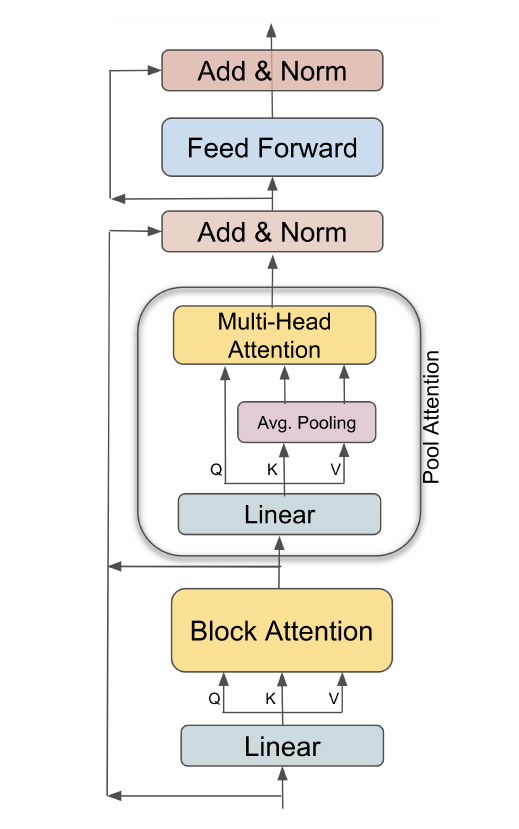
\includegraphics[height=8cm]{pooling_attention.png}
	\end{center}
	\caption{ لایه خودتوجهی تقویت شده ادغام شده \cite{Xiong2022AdaptingPT}}
	\label{fig:attention_pooling}
	\medskip
	\small
\end{figure}
کارهای تحقیقاتی در زمینه ی یادگیری تقویتی\LTRfootnote{reinforcement learning}
و پردازش زبان طبیعی در سال‌های اخیر رشد کرده است. در یادگیری تقویتی  یک عامل با محیط تعامل می‌کند و با آزمون و خطا، خط مشی بهینه را برای تصمیم گیری متوالی برای به حداکثر رساندن پاداش تجمعی آینده می‌آموزد. این پاداش می‌تواند یک معیار تعریف شده توسط توسعه دهنده بر اساس کار در حال حل باشد. در خلاصه‌سازی خودکار انتزاعی متن، نمونه‌هایی از چنین پاداش‌هایی ممکن است شامل حفظ برجستگی، مستلزم منطقی هدایت‌شده، و غیر افزونگی باشد. به طور کلی،  یادگیری تقویتی  در چهار حوزه مختلف برای بهبود خلاصه‌سازی خودکار استفاده می‌شود:

\section{روش‌های مبتنی بر یادگیری تقویتی}
\subsection{ یادگیری تقویتی برای حل چالش‌های مدل دنباله به دنباله عمیق}

استفاده از یادگیری تقویتی به منظور حل مسائل گوناگونی که مدل‌های دنباله به دنباله عمیق قادر به حل آن‌ها نیستند، امکانات بیشتری را فراهم می‌کند. به عنوان مثال، مشکلاتی مانند کمبود نوآوری در ایجاد خلاصه‌های خلاقانه و آموزنده و کاهش کیفیت خلاصه‌ها در صورت افزایش طول مقالات منبع، با استفاده از سیستم‌های یادگیری تقویتی و یادگیری خط‌مشی\LTRfootnote{ policy learning} بهبود یافته است.
علاوه بر این  مدل‌های دنباله به دنباله عمیق را نمی‌توان برای خلاصه کردن طیف گسترده ای از اسناد استفاده کرد، زیرا مدلی که بر روی یک مجموعه داده آموزش داده می‌شود، در یک مجموعه داده دیگر به خوبی عمل نمی‌کند و قابلیت تعمیم ندارد. رویکردهای مبتنی بر یادگیری تقویتی می‌تواند این  مشکل را با استفاده ازگرادیان خط مشی انتقادی \LTRfootnote{self-critic policy gradient}
و ترکیب آن با یادگیری انتقالی\LTRfootnote{Transfer Learning (TL) }
برای انتقال دانش از یک مجموعه داده به مجموعه دیگر برطرف کنند\cite{DeepTL_RL}.

فریم‌ورک پوبرل\LTRfootnote{PoBRL}
(ترکیب سیاست‌ها با حداکثر ارتباط حاشیه‌ای و یادگیری تقویتی) اهمیت، ارتباط و طول خلاصه را در زمینه خلاصه‌سازی چند سندی با جدا کردن مسئله بهینه‌سازی چند هدفه به مسائل فرعی کوچک‌تر که با استفاده از یادگیری تقویتی قابل حل هستند، بهینه می‌کند. 
اهمیت، ارتباط و طول خلاصه را در زمینه خلاصه‌سازی چند سندی با جدا کردن مسئله بهینه‌سازی چند هدفه به مسائل فرعی کوچک‌تر که قابل حل هستند، بهینه می‌کند.
این فریم‌ورک از الگوریتم حداکثر ارتباط حاشیه ای\LTRfootnote{ Maximal Marginal Relevance (MMR)}
برای استخراج اطلاعات مهم از اسناد استفاده می‌کند. استفاده از این الگوریتم باعث افزایش ارتباط بین  جملات و کاهش افزونگی می‌شود.
در ادامه با از یادگیری تقویتی رای بهینه سازی هر هدف به صورت جداگانه استفاده می کند و خط مشی های جداگانه ای را برای اهمیت، ارتباط و طول می آموزد\cite{PoBRL}.
خلاصه‌سازی چند سندی شامل سر و کار داشتن با اطلاعات پیچیده و همپوشانی از منابع متعدد است. الگوریتم‌های یادگیری تقویتی می‌توانند با مدل‌سازی خلاصه‌سازی به عنوان یک فرآیند تصمیم‌گیری متوالی  پیچیدگی را مدیریت کنند و یاد بگیرند جملات مرتبط حاوی اطلاعات را برای خلاصه انتخاب کنند. علاوه بر این  یادگیری تقویتی امکان بهینه‌سازی همزمان اهداف متعدد مانند اهمیت، افزونگی و طول را فراهم می‌کند و موجب برقراری تعادل بین اهداف و تولید خلاصه‌‌های مختصر، مرتبط و غیر تکراری شوند.

%در مرحله بعد، چارچوب از یادگیری تقویتی برای بهینه سازی هر هدف به صورت جداگانه استفاده می کند. خط مشی های جداگانه ای را برای اهمیت، ارتباط و طول می آموزد.
%چارچوب مبتنی بر یادگیری تقویتی برای خلاصه سازی چندسندی است که برای بهبود ارتباط بین جملات  و گنجاندن مطالب با اهمیت در خلاصه‌ی خروجی ارائه شده است.این چهارجوب با
سلیکیلماز\LTRfootnote{Celikyilmaz}
و همکاران مدل کدگذار-کدگشای چندعامله را برای بهبود خلاصه‌سازی اسناد طولانی با استفاده از عامل تعامل‌کننده\LTRfootnote{communicating agent}
ارائه کرده‌اند. این مدل وظیفه کدگذاری یک متن طولانی را بین چندین عامل همکاری تقسیم می‌کند، که هر کدام مسئول یک زیربخش از ورودی هستند. این عوامل برای به اشتراک گذاشتن اطلاعات پایه‌ی جامع و ایجاد یک خلاصه متمرکز و منسجم با یکدیگر ارتباط برقرار می‌کنند.  مدل ارائه شده در مقایسه با سایر مدل‌ها عملکرد بهتری دارد و خلاصه‌سازی اسناد طولانی با مدل‌های دنباله به دنباله را بهبود می‌بخشد.
\subsection{یادگیری تقویتی برای ترکیب خلاصه‌های استخراجی و انتزاعی} 
از یادگیری تقویتی برای ترکیب ویژگی‌های استخراجی با خلاصه انتزاعی برای استفاده از هر دو نوع خلاصه ی خودکار با الهام از رفتار انسان استفاده می‌شود. این مدل‌ها ابتدا برجسته‌ترین جملات را از سند ورودی استخراج می‌کنند، سپس با استفاده از دو شبکه: شبکه‌های استخراج‌کننده و انتزاعی، آنها را انتزاع می‌کنند. به عنوان مثال لیو\LTRfootnote{Liu}
و همکاران یک چارچوب متخاصم را پیشنهاد می‌کنند که مدل‌های انتزاعی و استخراجی را همزمان با استفاده از گرادیان خط ‌مشی برای بهینه‌سازی مدل انتزاعی برای خلاصه‌ای با پاداش بالا، آموزش می‌دهد که منجر به خلاصه‌ای منسجم‌تر می‌شود\cite{liu2018generative}.
همچنین چن و بانسال\LTRfootnote{Chen and Bansal}
یک مدل خلاصه‌سازی سریع پیشنهاد کردند که جملات برجسته را استخراج می‌کرد و سپس با استفاده از گرادیان خط مشی سطح جمله مبتنی بر یادگیری‌تقویتی بازنویسی می‌کرد\cite{chen2018fast}.
کریسینسکی \LTRfootnote{Kryscinski}
و همکاران  دو روش برای افزایش سطح انتزاع در خلاصه سازی  پیشنهاد می‌کنند: تجزیه رمزگشا به یک شبکه متنی و یک مدل زبانی از پیش آموزش‌دیده، و بهبود معیار جدید از طریق یادگیری خط‌مشی.
تکنیک اول شامل یک شبکه‌ی محتوایی\LTRfootnote{contextual network}
و یک مدل زبانی از پیش آموزش دیده است. شبکه‌ی محتوایی  بخش‌های مرتبط از سند منبع را بازیابی کرده و آنها را فشرده می‌کند. مدل زبان از پیش آموزش حاوی دانش قبلی در مورد تولید زبان است. این تفکیک مسئولیت ها امکان استخراج بهتر و تولید جملات مختصر را فراهم می کند.
تکنیک دوم شامل معرفی یک معیار جدید است که از طریق یادگیری خط مشی بهینه می‌شود. این معیار مدل را به تولید عبارات بدیع که در سند   منبع وجود نداشته‌اند تشویق می‌کند. با ترکیب این معیار جدید با معیار روژ که همپوشانی کلمات را با خلاصه حقیقت پایه اندازه گیری می‌کند، مدل قادر به تولید خلاصه‌های انتزاعی با عملکرد بالا در همپوشانی کلمات می‌شود \cite{kryscinski-etal-2018-improving}.

\subsection{یادگیری تقویتی  برای ایجاد معیارها و پاداش‌های جدید}

خلاصه‌سازی اسناد، مانند سایر کارهای مولد زبان،  اغلب به دلیل استفاده از اهداف آموزشی مبتنی بر  درست‌نمایی بیشینه\LTRfootnote{maximum likelihood}
مورد انتقاد قرار گرفته است.
درست‌نمایی بیشینه کیفیت خلاصه‌ی تولید شده را در نظر نمی‌گیرد و ممکن است خلاصه‌هایی تولید کند که فقط یک کپی از اسناد ورودی هستند یا پر از کلمات بی‌معنی هستند. به همین دلیل، یادگیری تقویتی به عنوان جایگزینی برای بهینه‌سازی مستقیم مدل‌ها بر روی معیارهای ارزیابی و پاداش صریح به کیفیت پیش‌بینی‌های مدل استفاده شده است	\cite{Parnell2022AMC}. 
معیارهای ارزیابی خلاصه‌سازی مانند روژـ۱\LTRfootnote{ROUGE-1}
،روژ-۲\LTRfootnote{ROUGE-2}،
روژ-‌ال\LTRfootnote{ROUGE-L}
و امتیازبرت\LTRfootnote{BERTScore}
به عنوان پاداش در رویکردهای یادگیری تقویتی استفاده شده است. با این حال، پارنل و همکاران  استدلال می‌کند که استفاده از امتیازات روژ به عنوان پاداش، جنبه‌های مهم خلاصه‌سازی، مانند خوانایی، روان بودن و اشتراک اطلاعات بین اسنادی در خلاصه‌سازی چند سندی را نادیده می‌گیرد و یک پاداش پوشش اصلاح شده همراه با یک برآوردگر گرادیان سیاست مبتنی بر اصول (ریلکس )	 \LTRfootnote{modified coverage reward along with a principled policy gradient estimator (RELAX)}
را پیشنهاد می‌دهند\cite{Parnell2022AMC, ALOMARI}.
ریلکس یک برآوردگر گرادیان خط مشی\LTRfootnote{policy}
با واریانس کم و بدون سوگیری\LTRfootnote{bias}
است که برای مسائل یادگیری تقویتی با فضاهای کنش مداوم، مانند خلاصه‌سازی متن، مناسب است\cite{Grathwohl2017BackpropagationTT}.

در عبارت\ref {eq:relax} تابع زیان ارائه شده برحسب ریلکس نمایش داده شده است.
بخش اول این عبارت سیاست را به تولید خروجی‌هایی با پاداش مورد انتظار بالا و بخش دوم به تولید خروجی‌‌های مشابه خروجی‌های قبلی 
تشویق می‌کند.
%	  تشویق می‌کند تا خروجی‌هایی تولید کند که پاداش مورد انتظار بالایی دارند و بخش دوم سیاست را تشویق می‌کند تا خروجی‌هایی مشابه خروجی‌های تولید شده در گذشته تولید کند همچنین
در این عبارت
$ r $
نشان دهنده‌ی پاداش 
$  c_\phi(\tilde{z}) $
یک متغیر کنترلی از پارامترهای $ φ $ است که انتظار می‌رود با پاداش کاهش واریانس همبستگی داشته باشد.
$  p(yـs) $ 
احتمال دنباله مشاهده شده خروجی $ y_s $ است.
$ z $
دنباله نمونه‌های $Gumbel-Softmax  $ است.
$ \tilde{z} $
دنباله ای از نمونه‌ها از یک توزیع $ Gumbel-Softmax $ مشروط بر $ y_s $ است.


\begin{equation}
	\label{eq:relax}
	L_\text{$ RELAX $} = -[r - c_\phi(\tilde{z})]   \log p(y^{s}) \quad + c_\phi(z) - c_\phi(\tilde{z})
\end{equation}
%	  \todo{یک بار دیگه متغیرها رو چک کن}


\subsection{ یادگیری تقویتی برای ایجاد خلاصه متناسب با نیاز کاربر}
درخلاصه‌سازی متن، یادگیری تقویتی می‌تواند نقش مهمی به عنوان یک رویکرد پیشرفته برای ارائه خلاصه‌های متناسب با نیاز کاربر ایفا کند. با استفاده از یادگیری تقویتی، سیستم‌ها قادر به تحلیل و فهم متن‌ها و درک نیازهای کاربران می‌شوند، سپس با اعمال تصمیمات متناسب، خلاصه‌هایی ایجاد می‌کنند که بیان کننده اصلی‌ترین اطلاعات و مفاهیم موجود در متن اصلی هستند. این رویکرد توانایی ارائه خلاصه‌های متناسب با نیازهای کاربر را بهبود می‌بخشد و تجربه خواندن و درک محتوای متن را بهبود می‌بخشد. همچنین، با استفاده از یادگیری تقویتی، سیستم‌ها قادر به بهبود خودکار خلاصه‌سازی و افزایش کیفیت خلاصه‌های تولید شده هستند. %\todo{تغیر کنه}
%\todo{مقدمه میخواد}
سایر روش‌های خلاصه‌سازی به کاربران اجازه نمی‌دهند، سلیقه‌ی خود را برای کنترل  جنبه‌های مختلف خلاصه‌های تولیدشده نشان بدهند. 

مدل کنترل‌سام
\LTRfootnote{controlSum}
با  افزودن توکن‌های کنترلی به ابتدای متن ورودی و استفاده از یک مدل کدگذار-کدگشا به کاربران اجازه‌ی اعمال ویژگی‌های مورد نیازهای خود بر خلاصه را می‌دهند. به عنوان مثال برای کنترل طول خلاصه خروجی ده طول مجزا تعریف می‌شود و هریک توکن‌های کنترلی نشانگر  یکی از این طول‌ها هستند. هدف آموزش این مدل از طریق تابع زیان درست‌نمایی بیشینه \LTRfootnote{maximum liklihood loss}
است  \cite{fan-etal-2018-controllable}. این هدف آموزش هیچ سیگنال نظارتی صریحی ندارد.
برای حل این مشکل چان  \LTRfootnote{Chan}
و همکاران
با اعمال محدودیت بر روی هدف آموزشی با استفاده از فرآیند تصمیم‌گیری مارکوف محدود  \LTRfootnote{Constrained Markov Decision Process (CMDP)}
یک چهارچوب خلاصه سازی پیشنهاد کرده‌اند که شامل یک تابع پاداش همراه با مجموعه‌ای از  محدودیت ها است و کنترل خلاصه سازی را تسهیل می‌کند. 
هدف عامل بیشینه کردن  پاداش مورد انتظار در عین اعمال محدودیت بر هزینه‌ها است. 
با داشتن این هدف، تصمیم‌گیرنده سعی می‌کند سیاستی را انتخاب کند که منجر به بیشینه کردن پاداش کلی تجمعی در طول زمان شود، در حالی که محدودیت‌ها بر هزینه‌ها رعایت شوند.
این هدف مدل را تشویق می‌کند که خلاصه‌ای شبیه خلاصه‌ی تولید شده توسط انسان تولید کند. با استفاده از این مدل کاربران می‌توانند طول ، مبزان فشردگی و محتوای خلاصه را کنترل کنند به عنوان مثال توضیحات یک محصول را به گونه‌ای خلاصه کند که در یک محدودیت کلمه در تبلیغات آنلاین قرار گیرد.
برای تبدیل مسئله محدود به مسئله بدون محدودیت   از ساده‌سازی لاگرانژ \LTRfootnote{Lagrangian relaxation}
و برای بهینه سازی از الگوریتم بهینه سازی مبتنی بر گرادیان، مانند ادام استفاده می‌شود.
برای اندازه‌گیری شباهت بین خلاصه خروجی و  مرجع بر اساس تعبیه‌های متنی برت
به عنوان تابع پاداش از امتیازبرت‌ استفاده می‌شود. 
برای کنترل تمرکز خلاصه بر روی یک موجودیت نامدار  \LTRfootnote{named entity}
ابتدا ارجاع موجودیت نامدار به سند اضافه می‌شود سپس یک محدودیت سوال و جواب اعمال می‌شود. 
این محدودیت بر روی امتیاز اف‌‌-۱ خروجی یک مدل سوال جواب که ورودی آن شامل یک سوال راجع به موجودیت نامدار و خلاصه‌ی تولید شده است اعمال می‌شود. 
علاوه بر این دو محدودیت عدم تکرار ترای‌گرم  \LTRfootnote{trigram}
و موجودیت‌های درخواستی برای افزایش خوانایی و کاهش تکرار در متن اعمال می‌شود.
%این محدودیت شامل یک سوال راجع به موجودیت نامدار و خلاصه‌ی تولید شده است که به عنوان ورودی به یک مدل سوال و جواب داده می‌شود و امتیاز اف‌‌-۱ ‌برای خروجی مدل محاسبه می‌شود.
مدل اینت‌سام    \LTRfootnote{IntSumm}
یک مدل خلاصه‌سازی تعاملی با هدف خلاصه کردن اطلاعات مهم بر اساس کوئری‌های \LTRfootnote{query}
کاربر و ارائه کوئری پیشنهادی برای کمک به کاربران است. در ابتدا این مدل یک خلاصه‌ی اولیه تولید می‌‌کند و به کاربر نمایش می‌دهد سپس یک کوئری از کاربر دریافت می‌کند و خلاصه‌ی اولیه به همراه پاسخ کوئری را به کاربر نمایش می‌دهد.
برای ارزیابی مدل ارائه شده مساحت منحنی بازیابی  \LTRfootnote{recall}
بر اساس طول خلاصه معرفی شده است که ستون عمودی آن امتیاز بازیابی روژ و ستون افقی آن طول خلاصه مرجع می‌باشد و مساحت بیشتر زیر منحنی نشان دهنده‌ی مدل بهتر است. یک نمونه از این نمودار در شکل \ref{fig:recall_curve}   نمایش داده شده است
\cite{shapira-etal-2021-extending}.


\begin{figure}[!h]
	\begin{center}
		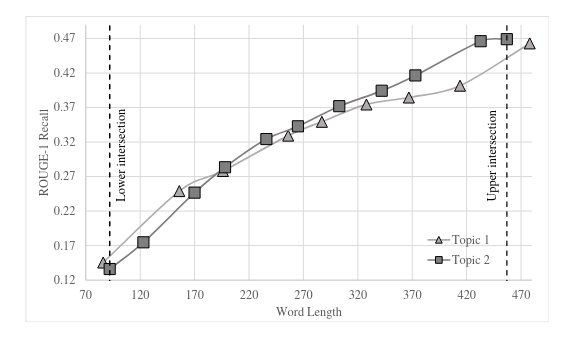
\includegraphics[height=8cm]{recall cureve.png}
	\end{center}
	\caption{ یک نمونه از نمودار منحنی بازیابی بر اساس طول \cite{shapira-etal-2021-extending}}
	\label{fig:recall_curve}
	\small{این نمودار دو تعامل متفاوت با سیستم خلاصه‌سازی را مقایسه می‌کند. هر نقطه نمایانگر   خروجی هر مرحله تعامل با کاربر است.}
	\medskip
	
\end{figure}




شاپیرا و همکاران برای بهبود مدل اینت‌سام و بهبود سرعت عمل در پاسخ‌گویی، توانایی پردازش کامل متون طولانی و رعایت تعادل میان اطلاعات کلی مقاله و اطلاعات مورد نیاز کاربر یک مدل جدید ارائه داده‌‌اند.
ورودی این مدل  مجموعه‌ی اسناد، کوئری و تاریخچه‌ی تعاملات با کاربر به همراه خروجی‌ قبلی است.
در ابتدا تعبیه کوئری به تعبیه اسناد ورودی الحاق شده  سپس امتیاز $ qMMR $ با استفاده از مدل $ RL-MMR $ ‌محاسبه می‌شود. هدف این امتیاز  ایجاد خلاصه‌ای شبیه به اسناد ورودی و کوئری و متفاوت از تاریخچه است.
سپس با استفاده از مکانیزم توجه با مرکزیت دوگانه  \LTRfootnote{two hub attention}
بر اساس کدگذاری به دست آمده از تاریخچه و مدل $ RL-MMR $ ‌

توزیع احتمال هر جمله را به دست ‌می‌آید.
مدل ام‌سام\LTRfootnote{MSumm}
یک مدل خودرگرسیون\LTRfootnote{Autoregressive}
است  که برای آموزش آن از یادگیری تقویتی به همراه مکانیسم پاداش دوگانه استفاده می‌شود.   معیار دلتا-روژ\LTRfootnote{Delta-ROUGE}
برای سنجش میزان اطلاعات اضافه‌ی خروجی نسبت به خروجی‌های قبلی و شباهت واژگانی و معنایی  برای سنجش میزان شباهت خروجی به کوئری به عنوان پاداش استفاده شده‌اند.
مدل $ RL-MMR $ ‌ موجب افزایش سرعت پردازش اطلاعات در مدل و پردازش کامل مجموعه‌ی اسناد و مکانیزیم پاداش دوگانه  تعادل موجب ایجاد تعادل اطلاعات می‌شود.    ساختار مدل در شکل  \ref{fig:MSumm}  نشان داده شده است
\cite{shapira-etal-2022-interactive}.
% برای پردازش سریع و کامل متون از مدل $ RL-MMR $ ‌و برای رعایت تعادل از یک مکانیسم پاداش دوگانه  (میزان شباهت خروجی به کوئری و میزان اطلاعات اضافه‌ی خروجی نسبت به خروجی‌های قبلی )استفاده شده است. 


\begin{figure}[!h]
	\begin{center}
		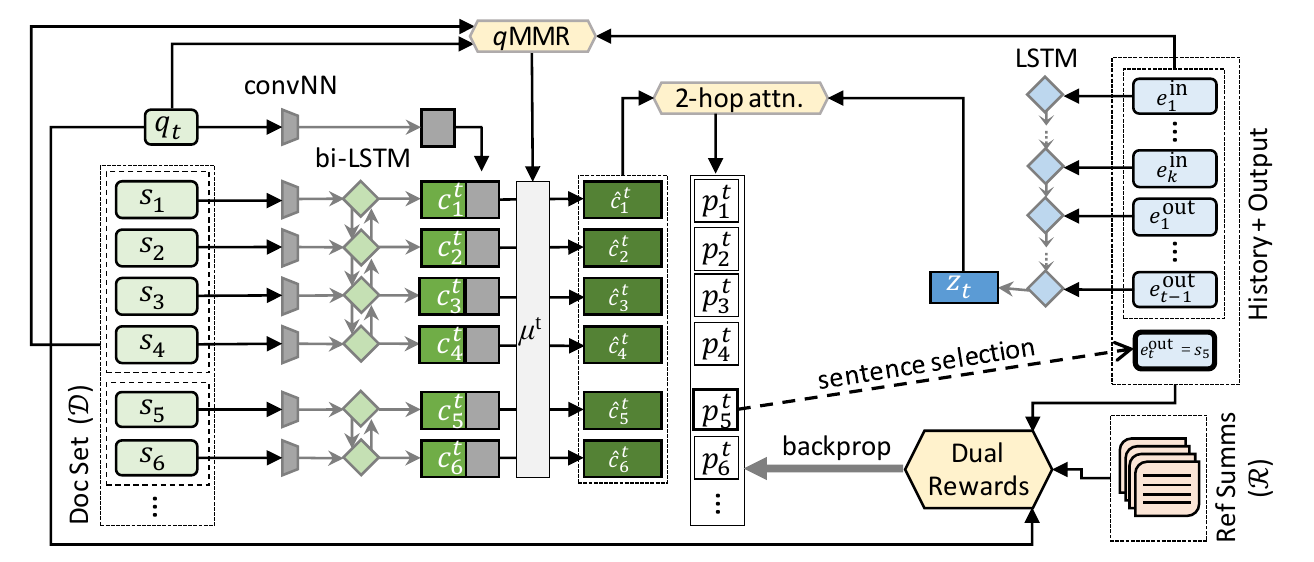
\includegraphics[height=7cm]{query-assited.png}
	\end{center}
	\caption{ معماری مدل  ام‌سام \cite{shapira-etal-2022-interactive}} 
	\label{fig:MSumm}
	
	\medskip
	
\end{figure}


%  ایجاد معیارهای جدید ارزیابی براساس منابعی غیر از خلاصه‌های مبنایی2. معیار روژ   دارای سه محدودیت اصلی است: تعصب آن نسبت به شباهت واژگانی، توجه کم آن به روان بودن و خوانایی خلاصه‌های انتزاعی تولید شده ، و پیش نیاز سخت آن برای استفاده از خلاصه‌های حقیقت پایه برای تولید امتیازات. علاوه بر این، خلاصه‌های تولید شده با معیار روژ بالا معمولاً جذابیت انسانی پایینی دارند ، بنابراین، محققان معیارهای جدیدی را برای افزایش تازگی [16]، سازگاری واقعی[17] و کیفیت بر اساس پاسخ به پرسش و رتبه‌بندی انسانی [17] با استفاده از رویکردهای پاداش‌دهی یادگیری تقویتی بدون نیاز به خلاصه‌های مبنایی ایجاد کردند.




%استفاده از برآورد درست‌نمایی بیشینه  در مدل‌های خلاصه‌سازی  ممکن است  با. به همین دلیل، یادگیری تقویتی به عنوان جایگزینی برای بهینه‌سازی مستقیم مدل‌ها بر روی معیارهای ارزیابی و پاداش صریح به کیفیت پیش‌بینی‌های مدل استفاده شده است. 


%مدل ‌$ awsome  $ با استفاده از 
برای متون طولانی یک روش بهینه ارائه میدهد.
مدل $ AWESOME $ از یک روش جدید دو مرحله‌ای برای بهبود خلاصه سازی متون طولانی استفاده می‌کند: استفاده از حافظه خارجی و شناسایی مفاهیم برجسته در کل سند
\LTRfootnote{global salient content identification}
. حافظه‌های خارجی در طول فرآیند خلاصه سازی قابل دسترسی هستند و بخش‌های کدگذاری شده سند و خلاصه‌های مربوط به آن‌ها را ردیابی می‌کنند تا درک جامع عمیق‌تر و انسجام خلاصه را تقویت کنند. علاوه بر این، محتوای برجسته‌ی جامع از بخش‌های گذشته و آینده استخراج می‌شود تا هر بخش را در حین کدگذاری تقویت کند و اطمینان حاصل شود که موضوعات مهم در خلاصه مورد توجه قرار می‌گیرند. با بهره‌گیری از این مکانیزم‌ها و یک معماری مبتنی بر حافظه کارآمد، این روش در زمینه‌های اطلاعاتی، انسجام و وفاداری نسبت به روش‌های قبلی عملکرد بهتری دارد
\ref{Cao2023AWESOMEGM}.
\section{روش های مبتنی بر مدل‌های زبانی بزرگ و چالش‌ها}
\subsection{توهم در مدل ‌های زبانی بزرگ}
 زیوی جی و همکارانش به بررسی مسئله توهم در مدل‌های زبان بزرگ پرداخته‌اند، پدیده‌ای که در آن مدل‌ها اطلاعاتی نامعتبر یا غیرواقعی تولید می‌کنند. این پژوهش با تمرکز بر کاربردهای پزشکی، روشی تعاملی مبتنی بر خودبازتابی ارائه می‌دهد که از طریق یک چرخه تکراری تولید، امتیازدهی و اصلاح، اعتبار پاسخ‌ها را افزایش می‌دهد. آزمایش‌های انجام شده نشان‌دهنده کاهش قابل توجه توهم و افزایش قابلیت اطمینان سیستم‌ها در پاسخگویی به سوالات پزشکی است\cite{ji-etal-2023-towards}​.

. ییجون شیاو و همکارانش رابطه بین توهم و عدم‌قطعیت پیش‌بینی در تولید زبان شرطی را بررسی کرده‌اند. آن‌ها با تاکید بر نقش مهم عدم‌قطعیت اپیستمیک، روشی برای بهبود الگوریتم جستجوی پرتو پیشنهاد می‌دهند که با کاهش عدم‌قطعیت، میزان توهمات تولید شده توسط مدل را کاهش می‌دهد. این پژوهش در وظایفی مانند توصیف تصویر و تولید داده به متن انجام شده و نتایج مثبت قابل توجهی در کاهش محتوای غیرواقعی نشان داده است\cite{xiao-wang-2021-hallucination}.

 دنیل کینگ و همکارانش روشی به نام $PINOCCHIO$ برای بهبود انسجام سیستم‌های خلاصه‌سازی انتزاعی ارائه داده‌اند. این روش با اعمال محدودیت‌هایی در جستجوی پرتو، تولید خروجی‌هایی را که به منبع متن مرتبط نیستند کاهش می‌دهد. نتایج آزمایش‌ها نشان داده که این رویکرد می‌تواند انسجام متون تولید شده را به طور قابل توجهی افزایش داده و توهمات را کاهش دهد، بدون آنکه بر روانی متن تاثیر زیادی بگذارد\cite{king-etal-2022-dont}​.

، جاشوا ماینز و همکارانش به بررسی مسئله توهم در خلاصه‌سازی انتزاعی اسناد پرداخته‌اند. آن‌ها نشان می‌دهند که مدل‌های تولید متن شرطی اغلب محتوایی تولید می‌کنند که با متن منبع سازگار نیست و این پدیده را به عنوان "توهم درونی" و "توهم بیرونی" طبقه‌بندی می‌کنند. این مقاله از طریق ارزیابی انسانی نشان می‌دهد که بیش از 70٪ خلاصه‌ها شامل محتوای توهم‌آمیز هستند که اکثریت آن‌ها به‌ویژه در توهم بیرونی، نادرست می‌باشند. نویسندگان همچنین پیشنهاد می‌کنند که مدل‌های از پیش آموزش‌دیده مانند $BERTS2S$ نسبت به مدل‌های دیگر، خلاصه‌های دقیق‌تر و با توهم کمتر تولید می‌کنند. این پژوهش با ارائه معیارهایی جدید برای ارزیابی دقت و اعتبار خلاصه‌ها، مسیر بهتری برای بهبود ارزیابی‌های خودکار و روش‌های تولید خلاصه‌سازی باز می‌کند​\cite{maynez-etal-2020-faithfulness}.
 جورج کریسوستومو و همکارانش تأثیر هرس مدل‌های زبان بزرگ بر کاهش توهم در خلاصه‌سازی متون را بررسی کرده‌اند. آن‌ها با استفاده از روش‌های پیشرفته هرس، مانند $SparseGPT$ و $Wanda$، نشان داده‌اند که مدل‌های هرس‌شده نسبت به مدل‌های اصلی توهم کمتری دارند. این مدل‌ها بیشتر بر متن منبع تکیه کرده و خلاصه‌هایی با همپوشانی واژگانی بالاتر و محتوای واقع‌گرایانه‌تر تولید می‌کنند. آزمایش‌ها روی پنج مجموعه داده مختلف و چندین مدل، کاهش قابل‌توجه ریسک توهم را با افزایش میزان هرس نشان داده است. این پژوهش، استفاده از مدل‌های هرس‌شده را به‌عنوان راهکاری مؤثر برای کاهش توهم در خلاصه‌سازی پیشنهاد می‌کند.
 
مسئله توهم در مدل‌های زبان بزرگ یکی از چالش‌های اساسی در تولید زبان طبیعی است که می‌تواند اعتبار و اطمینان به این مدل‌ها را تحت تأثیر قرار دهد. استفاده از روش‌های مبتکرانه و دقیق می‌تواند به طور قابل توجهی میزان توهم را کاهش داده و انسجام و دقت خروجی‌های مدل را بهبود بخشد. این پیشرفت‌ها راه را برای استفاده ایمن‌تر و موثرتر از مدل‌های زبان در کاربردهای حساس، از جمله پزشکی و خلاصه‌سازی متون، هموار می‌کند.

\subsection{هرس مدل های زبانی}

در حوزه بهینه‌سازی مدل‌های زبانی بزرگ، روش‌های مختلفی برای کاهش پیچیدگی محاسباتی و منابع مورد نیاز ارائه شده‌اند.
فانگ و همکاران الگوریتمی برای هرس ساختاریافته مدل‌های زبانی بزرگ ارائه داده‌اند که با وابستگی کمتر به داده، نیازی به مجموعه داده کامل ندارد و در مدت کوتاهی قابل اجرا است. الگوریتم $LLM-Pruner$ شامل سه مرحله کلیدی است: ابتدا وابستگی بین اجزای مدل شناسایی می‌شود، سپس اهمیت هر بخش وابسته به‌صورت مستقل از وظایف \LTRfootnote{task-agnostic} ارزیابی می‌شود و در نهایت، با استفاده از روش لورا، عملکرد مدل با حداقل داده بازیابی می‌شود. این روش توانسته با هرس ۲۰ درصد از مدل، ۹۴ درصد از کارایی اولیه را حفظ کند. نتایج این تحقیق نشان می‌دهد که رویکرد پیشنهادی با شناسایی و هرس بخش‌های وابسته مدل به صورت داده‌محور و بدون نیاز به به‌روزرسانی وزن‌ها، روشی کارآمد و سریع برای کاهش پیچیدگی مدل‌های زبانی بزرگ ارائه می‌دهد\cite{men2024shortgpt}.


 ژانگ و همکاران  الگوریتم $D-PRUNER $را معرفی کرده‌اند. این الگوریتم با هدف ارائه یک روش هرس داده‌محور و غیرساختاری طراحی شده که ضمن حفظ دانش عمومی مدل، توانایی آن را در فهم دانش دامنه خاص نیز حفظ کند. رویکرد $D-PRUNER$ در سه مرحله کلیدی شامل شناسایی اهمیت وزن‌های عمومی، بهینه‌سازی تابع ضرر با اضافه کردن  عبارت منظم‌سازی     \LTRfootnote{regularization term} برای جلوگیری از تغییر وزن‌های مهم، و در نهایت هرس وزن‌های کم‌اهمیت با استفاده از "فیشر تجربی" پیاده‌سازی می‌شود. نتایج این تحقیق نشان می‌دهد که این روش نه تنها پیچیدگی محاسباتی مدل را کاهش می‌دهد، بلکه با حفظ توازن میان دانش عمومی و خاص، عملکرد مدل را در دامنه‌های تخصصی بهبود می‌بخشد و نرخ سردرگمی \LTRfootnote{perplexity} کمتری نسبت به روش‌های دیگر ارائه می‌دهد\cite{zhang2024pruning}.

یکی از پژوهش‌های کلیدی در زمینه کاهش پیچیدگی مدل‌های زبانی بزرگ، مقاله‌ای از $Xin Men$ است. این تحقیق بر شناسایی  اضافه‌بودگی   \LTRfootnote{redundancy}در لایه‌های شبکه عصبی مدل‌های زبانی بزرگ تمرکز دارد. یافته اصلی نشان می‌دهد که بسیاری از لایه‌های میانی و انتهایی مدل تغییرات محدودی در حالات پنهان ایجاد می‌کنند و می‌توان آن‌ها را با حداقل تأثیر بر عملکرد مدل حذف کرد.

برای ارزیابی اهمیت هر لایه، متریک $Block Influence (BI)$ معرفی شده است. این متریک میزان تغییر حالات پنهان\LTRfootnote{hidden states} پس از عبور از هر لایه را می‌سنجد. $BI$ بر اساس شباهت کسینوسی بین ورودی و خروجی لایه تعریف شده است؛ به این صورت که $BI$ پایین‌تر نشان‌دهنده تغییرات کمتر و اهمیت کمتر لایه است.

با استفاده از این متریک، لایه‌های با $BI$ پایین شناسایی و حذف می‌شوند. این روش توانسته است با حذف ۲۵٪ از لایه‌های مدل، حدود ٪۹۰ از عملکرد اولیه را حفظ کند و در عین حال، از روش‌های پیشرفته دیگر در این زمینه پیشی بگیرد. همچنین، این روش با تکنیک‌های کوانتایزه‌سازی سازگار است و امکان کاهش بیشتر محاسبات و پارامترها را فراهم می‌کند.

\begin{equation}
	BI_i = 1 - \mathbb{E}_{X, t} \left[ \frac{X_{i,t}^\top X_{i+1,t}}{\|X_{i,t}\|_2 \|X_{i+1,t}\|_2} \right]
	\label{eq:bi}
\end{equation}

در این رابطه‌ی\ref{eq:bi} \( X_{i,t} \) نشان‌دهنده \( t \)-امین ردیف از حالات پنهان لایه \( i \) است. \( X_{i+1,t} \) نشان‌دهنده \( t \)-امین ردیف از حالات پنهان لایه \( i+1 \) است. \( \|\cdot\|_2 \) نُرم اقلیدسی را نشان می‌دهد و \( \mathbb{E}_{X, t} \) بیانگر امید ریاضی روی مقادیر \( X \) و \( t \) است. این متریک بر اساس شباهت کسینوسی بین ورودی و خروجی لایه عمل می‌کند. هرچه این شباهت بیشتر باشد (مقدار \( BI \) کمتر)، لایه تغییرات کمتری ایجاد کرده و اهمیت آن کاهش می‌یابد.


یکی از پژوهش‌های برجسته در زمینه کاهش پیچیدگی مدل‌های زبانی بزرگ، مقاله‌ای از یانگ ژانگ است که روش برش دقیق‌تر \LTRfootnote{FINERCUT} را برای هرس لایه‌های مدل‌های زبانی بزرگ ارائه می‌دهد. این روش برخلاف روش‌های پیشین، لایه‌های خودتوجهی\LTRfootnote{self-attention} و شبکه عصبی پیشخور\LTRfootnote{FFN} را به‌صورت جداگانه و مستقل به‌عنوان کاندیداهای هرس در نظر می‌گیرد. الگوریتم به‌صورت تکراری لایه‌هایی را که حذف آن‌ها کمترین تغییر را در خروجی مدل ایجاد می‌کنند، انتخاب و حذف می‌کند. برای اندازه‌گیری تغییرات خروجی، از معیارهای مختلفی مانند فاصله اقلیدسی، فاصله زاویه‌ای و واگرایی جنسن-شانون ($JSD$) استفاده می‌شود. معیار $JSD$، که برای سنجش شباهت بین توزیع‌های احتمالاتی طراحی شده، با در نظر گرفتن توزیع خروجی‌های مدل قبل و بعد از حذف یک لایه، به شناسایی لایه‌های کم‌اهمیت کمک می‌کند.

نتایج این روش نشان می‌دهد که با حذف ۲۵٪ از لایه‌های لاما 3-8$B$، ۹۰٪ از عملکرد مدل حفظ می‌شود و با حذف ۳۰٪ از لایه‌های لاما 3-70$B$، مدل توانسته است ۹۵٪ عملکرد اولیه را حفظ کند، بدون نیاز به تنظیم دوباره. همچنین، در لایه‌های انتهایی مدل، ترکیبی از حذف لایه‌های توجه و استفاده از لایه‌های متوالی شبکه تغذیه پیش‌رو، به ساختارهای کارآمدتری منجر شده است. این روش نه تنها عملکرد بهتری نسبت به روش‌های پیشرو ارائه می‌دهد، بلکه طراحی جدیدی برای معماری مدل‌های آینده پیشنهاد می‌کند که می‌تواند بازدهی بیشتری در استفاده از منابع محاسباتی داشته باشد\cite{zhang2024finercut}.



\subsection{توهم در خلاصه‌سازی}
یکی از مطالعات برجسته در زمینه کاهش توهم در مدل‌های زبانی بزرگ  و بهبود کیفیت خلاصه‌سازی انتزاعی متون طولانی، مقاله‌ای از یو شیا است. این تحقیق اولین چارچوب یادگیری فعال برای کاهش توهم در مدل‌های زبانی ارائه می‌دهد و بر روی تولید خلاصه‌های متنی با تأکید بر حفظ دقت معنایی متمرکز است. روش پیشنهادی، سه نوع خطای رایج شامل خطاهای چارچوب معنایی، خطاهای گفتمان، و خطاهای قابلیت تأیید محتوا را شناسایی کرده و از متریک‌های پیشرفته‌ای مانند $FactKB$، $UniEval$ و$ BERT-P$ برای ارزیابی این خطاها استفاده می‌کند.

الگوریتم $HADAS$، با رویکردی داده‌محور و متنوع‌محور، نمونه‌های داده‌ای را که شامل انواع مختلفی از توهمات هستند برای بهبود مدل انتخاب می‌کند. این انتخاب با استفاده از واگرایی جنسن-شانون ($JSD$) به منظور سنجش تنوع توزیع انواع توهمات انجام می‌شود. این روش نه تنها به طور مؤثری توهمات در خلاصه‌سازی‌های انتزاعی را کاهش داده است، بلکه کیفیت و دقت خلاصه‌های تولیدشده را نیز بهبود می‌بخشد. نتایج نشان می‌دهد که این چارچوب، با کاهش نیاز به حاشیه‌نویسی انسانی پرهزینه و ارائه روشی کارآمد برای هرس مدل، به‌طور خاص در زمینه خلاصه‌سازی متون طولانی تأثیرگذار است\cite{xia2024hallucinationdiversityawareactivelearning}.


 تایجی لی و همکارانش روش $SliSum$ را برای کاهش توهم و افزایش دقت در خلاصه‌سازی مدل‌های زبان بزرگ ارائه داده‌اند. این روش شامل سه مرحله کلیدی است:
\begin{itemize}
	\item 
تولید خلاصه‌های محلی با پنجره‌های لغزنده: متن منبع به بخش‌های همپوشانی‌شده تقسیم می‌شود (پنجره‌های لغزنده)، و مدل زبان برای هر پنجره یک خلاصه محلی تولید می‌کند. این همپوشانی‌ها کمک می‌کنند که متن به طور عادلانه در سراسر مقاله پردازش شود و مشکل سوگیری موقعیتی کاهش یابد.
\item 
خوشه‌بندی و فیلتر کردن بر اساس انسجام درونی: جملات تولیدشده در خلاصه‌های محلی با استفاده از الگوریتم خوشه‌بندی $Lexical$ (مانند $DBSCAN$) تجزیه و تحلیل می‌شوند. جملات مرتبط با یک رویداد مشخص در یک خوشه قرار می‌گیرند و جملات کم‌اهمیت یا ناسازگار حذف می‌شوند تا انسجام و دقت حفظ شود.
\item 
تجمیع و تولید خلاصه جامع: جملات منتخب از خوشه‌ها، با استفاده از رأی‌گیری اکثریتی و به ترتیب معنایی ترکیب می‌شوند تا یک خلاصه جامع و دقیق برای کل مقاله تولید شود. این مرحله همچنین از مدل زبان برای اطمینان از روانی و ساختارمند بودن متن استفاده می‌کند.
\end{itemize}
این رویکرد، بدون نیاز به تنظیم مجدد مدل یا منابع اضافی، باعث کاهش توهم و افزایش دقت و انسجام خلاصه‌های تولیدشده می‌شود و در متون کوتاه و بلند عملکردی مؤثر نشان می‌دهد. تصویر \ref{fig:slimsum} نشان‌دهنده مراحل مختلف این فرآیند است که شامل پردازش هر پنجره و ترکیب نتایج به روش ساختاریافته است\cite{li-etal-2024-improving-faithfulness}.

\begin{figure}[!h]
	\begin{center}
		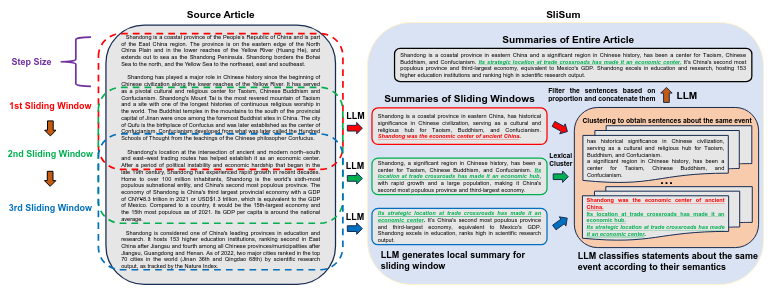
\includegraphics[height=5cm]{slimsum.png}
	\end{center}
	\caption{  رویکرد $SlimSum$ برای حل تضادهای معنایی در خلاصه‌سازی }
	\small{
		
		توضیح: تصویری از فرآیند $SlimSum$ که با رأی‌گیری اکثریت میان جملات هر خوشه بر اساس معنای آن‌ها، به حل مشکل تضاد معنایی در خلاصه‌سازی می‌پردازد. به عنوان مثال، جملات سبز دارای معنای مشابه هستند و دو بار ظاهر می‌شوند، در حالی که جمله قرمز با معنای متفاوت فقط یک بار ظاهر می‌شود. بنابراین، جمله دوم سبز برای خلاصه نهایی انتخاب می‌شود. $SlimSum$ مقالات منبع را در سطح جملات پردازش می‌کند و برای ساده‌تر کردن نمایش، پنجره‌های موجود در تصویر به صورت خطوط متنی نمایش داده شده‌اند\cite{li-etal-2024-improving-faithfulness}. }
	\label{fig:slimsum}
	
	\medskip
	
\end{figure}




\section{معیارهای ارزیابی خلاصه‌سازی خودکار}
در ارزیابی خلاصه‌سازی خودکار، هدف اصلی سنجش کیفیت و دقت خلاصه‌های تولید شده است. برای این منظور، معیارهای مختلفی طراحی شده‌اند که توانایی مدل‌ها در تولید خلاصه‌های دقیق، مفهومی و وفادار به متن اصلی را ارزیابی می‌کنند. این معیارها می‌توانند به صورت کمی و بر اساس مقایسه خلاصه‌های تولید شده با متن‌های مرجع، یا به‌طور کیفی با استفاده از تحلیل‌های معنایی و ساختاری عمل کنند. در این بخش، به معرفی و بررسی مهم‌ترین معیارهای ارزیابی در این حوزه مانند روژ، امتیاز برت ، فکت‌سی‌سی پرداخته می‌شود. این معیارها هرکدام از جنبه‌های مختلف کیفیت خلاصه‌ها را ارزیابی کرده و نقش مهمی در توسعه و بهبود الگوریتم‌های خلاصه‌سازی خودکار ایفا می‌کنند. همچنین، محدودیت‌های این معیارها در شناسایی هالوسینیشن و چالش‌های آن‌ها در سنجش وفاداری خلاصه‌ها نیز مورد بررسی قرار خواهد گرفت.
\begin{itemize}
	\item روژ
	 یکی از پرکاربردترین معیارهای ارزیابی در خلاصه‌سازی خودکار است که بر اساس تطابق کلمات یا عبارات $n-gram$ بین خلاصه تولیدشده و متن مرجع عمل می‌کند. روژ شاخص‌هایی مانند دقت \LTRfootnote{Precision} ، فراخوان \LTRfootnote{Recall} و $F1 $را برای شباهت زبانی محاسبه می‌کند. اگرچه این معیار در اندازه‌گیری شباهت‌های سطح کلمه مؤثر است، اما از درک معنایی عمیق و سنجش وفاداری محتوا ناتوان است. به عنوان مثال، $Zhou$ و همکاران نشان داده‌اند که اگر یک خلاصه شامل مقدار زیادی محتوای هالوسینیشن باشد، ممکن است همچنان روژ بالایی کسب کند.\cite{zhou-etal-2021-detecting,lin-2004-rouge}.
	\item 
	امتیاز برت برخلاف معیارهای سطح کلمه مانند روژ، از مدل‌های زبانی پیش‌آموزش‌دیده (مانند برت) برای اندازه‌گیری شباهت معنایی میان خلاصه تولیدشده و متن مرجع استفاده می‌کند. این معیار توانایی بیشتری در درک روابط زبانی پیچیده و شباهت معنایی عمیق دارد، اما همچنان در شناسایی دقیق هالوسینیشن‌ها محدودیت‌هایی دارد\cite{zhang-etal-2024-benchmarking}.
	\item 
	فکت‌سی‌سی مبتنی بر مدل‌های استنتاج متنی\LTRfootnote{Natural Language Inference(NLI)} طراحی شده و تمرکز آن بر بررسی میزان درستی و وفاداری اطلاعات موجود در خلاصه به متن اصلی است. فکت‌سی‌سی تلاش می‌کند تا محتواهای نادرست یا ناسازگار را شناسایی کند و از این طریق بهبودهایی در سنجش وفاداری ایجاد کند. این معیار نسبت به روژ و امتیازبرت توانایی بهتری در ارزیابی هالوسینیشن دارد\cite{factcc-etal-2020-evaluating}.
\end{itemize}
\subsection{محدودیت‌ها و پیشرفت‌ها}

اگرچه معیارهایی مانند روژ\LTRfootnote{rouge} و امتیازبرت\LTRfootnote{BERTScore} در اندازه‌گیری شباهت زبانی میان خلاصه‌ها و متن مرجع مؤثر هستند، اما توانایی لازم برای شناسایی هالوسینیشن را ندارند. هالوسینیشن به تولید محتوای نامرتبط، ساختگی یا ناسازگار با متن اصلی اشاره دارد که می‌تواند وفاداری خلاصه‌ها را کاهش دهد و اعتماد کاربران به خروجی مدل را به چالش بکشد.


پژوهش‌های اخیر، مانند $Maynez$ و همکاران روش‌های جایگزینی را معرفی کرده‌اند که مستقیماً هالوسینیشن را در سطح توکن شناسایی می‌کنند و به تحلیل دقیق‌تر ناهماهنگی‌های موجود در متن می‌پردازند. این پیشرفت‌ها با ارائه ارزیابی‌های جزئی‌تر، امکان بهبود قابل‌توجه در کیفیت و دقت خلاصه‌سازی انتزاعی را فراهم کرده‌اند\cite{maynez-etal-2020-faithfulness}.











\chapter{روش‌ارائه شده}


\chapter{نتایج}

 
 %این پژوهش استفاده از مدل‌های یادگیری عمیق، مدل‌های یادگیری تقویتی  و مدل‌های مبتنی بر ساختار در سیستم‌های خلاصه‌سازی انتزاعی را مورد بررسی قرار داد. هدف از این بررسی، درک پیشرفت‌ها و چالش‌های مرتبط و  رویکردهای ارائه شده برای بهبود کارایی سیستم‌های خلاصه‌سازی انتزاعی است.  در حال حاضر، تحقیقات خلاصه سازی انتزاعی  بر یافتن مؤثرترین و مناسب‌ترین مدل‌های از پیش آموزش دیده و چگونگی تطبیق بازنمایی‌های جامع به دست آمده از این مدل‌ها برای بهبود بیشتر کیفیت خلاصه‌ها و نزدیک‌تر کردن آنها به سطوح خلاصه‌سازی انسانی متمرکز است.
%\chapter{جمع‌بندی}
 به طور خلاصه در این پژوهش ما پیشرفت‌های اخیر خلاصه‌سازی متن انتزاعی را با استفاده از مدل‌های یادگیری عمیق، مدل‌های یادگیری تقویتی و مدل‌های مبتنی بر ساختار بررسی کرده‌ایم. ما در مورد رویکرد های مختلفی که پیشنهاد شده است و چالش هایی که هنوز باید پرداخته شوند، بحث کرده‌ایم.

مدل‌های یادگیری عمیق به ویژه هنگامی که با یادگیری تقویتی ترکیب شوند، برای خلاصه‌سازی متن انتزاعی  مؤثر هستند. با این که، آموزش این مدل‌ها  از نظر محاسباتی پرهزینه است و خلاصه‌ی تولید شده توسط این مدل‌های ممکن است  به اندازه خلاصه‌های نوشته شده توسط انسان روان یا آموزنده نباشد زیرا مدل‌های یادگیری عمیق بر روی مجموعه داده‌های بزرگی دادگان آموزش داده می‌شوند که جمع‌آوری و برچسب‌گذاری آن زمان‌بر و پرهزینه است.

مدل‌های مبتنی بر ساختار پتانسیل رفع برخی از محدودیت‌های مدل‌های یادگیری عمیق را دارند. این مدل‌ها می‌توانند دانش حوزه و قواعد زبانی را در خود جای دهند که می‌تواند به بهبود کیفیت خلاصه‌های تولید شده کمک کند. با این حال، آموزش این مدل ها دشوار است و قابل تعمیم به حوزه‌های جدید نیست.

به طور کلی، در سال های اخیر پیشرفت قابل توجهی در خلاصه سازی متن انتزاعی حاصل شده است و رویکردهای مختلفی برای کاهش افزونگی و افزایش خوانایی خلاصه‌ها ارائه شده است با این حال، هنوز چالش‌هایی زیادی وجود دارد.در حال حاضر، تحقیقات خلاصه سازی انتزاعی  بر یافتن مناسب‌ترین مدل‌های از پیش آموزش دیده و چگونگی تطبیق بازنمایی‌های به دست آمده از این مدل‌ها برای بهبود  کیفیت خلاصه‌ها و نزدیک‌تر کردن آن‌ها به  خلاصه‌سازی انسانی متمرکز است.


%--------------------------------------------------------------------------appendix( مراجع و پیوست ها)
\chapterfont{\vspace*{-2em}\centering\LARGE}%

\appendix
\bibliographystyle{plain-fa}
\bibliography{references}
%\chapter*{‌پیوست}
\markboth{پیوست}{}
\addcontentsline{toc}{chapter}{پیوست}
موضوعات مرتبط با متن گزارش پایان نامه كه در يكی از گروه‌های زير قرار می‌گيرد، در بخش پيوست‌ها آورده شوند:
\begin{enumerate}
\item  اثبات های رياضی يا عمليات رياضی طولانی‌.‌
\item داده و اطلاعات نمونه (های) مورد مطالعه (\lr{Case Study}) چنانچه طولانی باشد‌.‌
\item نتايج كارهای ديگران چنانچه نياز به تفصيل باشد‌.‌
\item مجموعه تعاريف متغيرها و پارامترها، چنانچه طولانی بوده و در متن به انجام نرسيده باشد‌.‌
\end{enumerate}
% براي شماره‌گذاري روابط، جداول و اشكال موجود در پيوست‌ از ساختار متفاوتي نسبت به متن اصلي استفاده مي‌شود كه در زير به‌عنوان نمونه نمايش داده شده‌است. 
% \begin{equation}
%F=ma
%\end{equation}
\section*{کد میپل }
\begin{latin}
\begin{verbatim}

with(DifferentialGeometry):
with(Tensor):
DGsetup([x, y, z], M)
																	frame name: M
a := evalDG(D_x)
																	D_x
b := evalDG(-2 y z D_x+2 x D_y/z^3-D_z/z^2)


\end{verbatim}
\end{latin}
%--------------------------------------------------------------------------dictionary(واژه نامه ها)
%اگر مایل به داشتن صفحه واژه‌نامه نیستید، خط زیر را غیر فعال کنید.
%\parindent=0pt
\chapter*{ واژه‌نامه‌ی انگلیسی به فارسی}
\pagestyle{style9}
\lhead{\thepage}\rhead{واژه‌نامه‌ی انگلیسی به فارسی}
\addcontentsline{toc}{chapter}{واژه‌نامه‌ی انگلیسی به فارسی}
\LTRmulticolcolumns
\begin{multicols}{2}
{\bf {ا}}
\farsiTOenglish{الگوریتم حداکثر سازی نقطه-محصول فرا یادگیری}{Meta-Learned Dot-Product Maximization}
\farsiTOenglish{امتیازبرت}{BERTScore}
\vspace*{3mm}
{\bf {ب}}
\farsiTOenglish{بارت}{BART}
\farsiTOenglish{بازنمایی}{Representation}
\farsiTOenglish{بازیابی}{recall}
\farsiTOenglish{بیگ‌برد}{Big‬‬ ‫‪Bird‬‬}
\vspace*{3mm}
{\bf {پ}}
\farsiTOenglish{پراکنده}{sparse}
\farsiTOenglish{پيش‌آموزش}{pretraining}
\farsiTOenglish{پگاسوس}{PEGASUS}
\vspace*{3mm}
{\bf {ت}}
\farsiTOenglish{تابع زیان درست‌نمایی بیشینه}{maximum liklihood loss}
\farsiTOenglish{ترای‌گرم}{trigram}
\farsiTOenglish{ترنسفورمر}{transformer}
\farsiTOenglish{تعبیه}{embedding}
\farsiTOenglish{تعبیه نشانه}{token embedding}
\farsiTOenglish{تنظیم}{regularization}
\farsiTOenglish{تنظیم دقیق پارامترها}{fine-tuning}
\farsiTOenglish{توالی}{sequence}
\farsiTOenglish{توجه با مرکزیت دوگانه}{two hub attention}
\farsiTOenglish{توجه به خود}{Self-attention}
\farsiTOenglish{توجه جامع}{global attention}
\farsiTOenglish{توسعه}{deploy}
\vspace*{3mm}
{\bf {ج}}
\farsiTOenglish{جامع}{global}
\farsiTOenglish{جملات فاصله‌افتاده}{gap‬‬ ‫‪sentences}
\farsiTOenglish{جي‌پي‌تي }{GPT}
\vspace*{3mm}
{\bf {چ}}
\farsiTOenglish{چند معنایی}{polysemy}
\vspace*{3mm}
{\bf {ح}}
\farsiTOenglish{حافظه‌ی بلند مدت طولانی}{long short-term memory networks(LSTM)}
\farsiTOenglish{حاوی اطلاعات مفید}{informative}
\farsiTOenglish{حداکثر ارتباط حاشیه ای}{ Maximal Marginal Relevance (MMR)}
\vspace*{3mm}
{\bf {خ}}
\farsiTOenglish{خط مشی}{policy}
\farsiTOenglish{خود رگرسیون}{Autoregressive}
\vspace*{3mm}
{\bf {د}}
\farsiTOenglish{درست‌نمایی بیشینه}{maximum likelihood}
\farsiTOenglish{درهم‌سازی حساس به مکان}{locality-sensitive‬‬ ‫‪hashing‬‬}
\farsiTOenglish{دلتا-روژ }{Delta-ROUGE}
\farsiTOenglish{دنسر}{Divide-and-ConquER (DANCER)}
\farsiTOenglish{دوسویه}{bidirectional}
\vspace*{3mm}
{\bf {ر}}
\farsiTOenglish{روژ-ال}{ROUGE-L}
\farsiTOenglish{روژـ1}{ROUGE-1}
\farsiTOenglish{روژـ2}{ROUGE-2}
\farsiTOenglish{ریلکس}{modified coverage reward along with a principled policy gradient estimator (RELAX)}
\vspace*{3mm}
{\bf {س}}
\farsiTOenglish{ساده‌سازی لاگرانژ}{Lagrangian relaxation}
\farsiTOenglish{سوگیری}{bias}
\vspace*{3mm}
{\bf {ش}}
\farsiTOenglish{شبکه‌های عصبی بازگشتی}{recurrent neural network (RNN)}
\vspace*{3mm}
{\bf {ع}}
\farsiTOenglish{عامل  }{agent}
\farsiTOenglish{عامل تعامل کننده}{communicating agent}
\farsiTOenglish{عبارت مقدمه و بدنه}{lead-and-body phrase}
\farsiTOenglish{عمل }{task}
\farsiTOenglish{عمل پايين‌دست}{downstream task}
\vspace*{3mm}
{\bf {ف}}
\farsiTOenglish{فرا یادگیری}{Meta-Learning}
\vspace*{3mm}
{\bf {ک}}
\farsiTOenglish{کوئری}{query}
\vspace*{3mm}
{\bf {ل}}
\farsiTOenglish{لایه‌های برگشت‌پذیر}{reversible layers}
\vspace*{3mm}
{\bf {م}}
\farsiTOenglish{متقاطع زبانی}{cross-lingual}
\farsiTOenglish{مجموعه‌ی دادگان}{corpus}
\farsiTOenglish{مدل موضوعی عصبی}{Neural Topic Model(NTM}
\farsiTOenglish{مدل مولد نقطه‌ای}{Pointer-Generator model}
\farsiTOenglish{مکانیرم توکن سراسری}{Global-token mechanism}
\vspace*{3mm}
{\bf {ن}}
\farsiTOenglish{نمایش نهفته}{latent representation}
\vspace*{3mm}
{\bf {و}}
\farsiTOenglish{واحد بازگشتی دروازه‌ای}{gated recurrent unit (GRU)}
\farsiTOenglish{وظایف}{tasks}
\farsiTOenglish{وظایف پایین‌دست}{downstream tasks}
\vspace*{3mm}
{\bf {ه}}
\farsiTOenglish{هدف آموزش}{training objective}
\farsiTOenglish{هستان‌شناسی}{ontology}
\farsiTOenglish{هم‌پوشانی بلوک‌های توجه}{Overlapping attention windows}
\vspace*{3mm}
{\bf {ی}}
\farsiTOenglish{یادگیری تقویتی}{reinforcement learning}
\farsiTOenglish{یادگیری خط مشی }{policy learning }
\vspace*{3mm}
\end{multicols}%
\chapter*{ واژه‌نامه‌ی انگلیسی به فارسی}
\pagestyle{style9}
\lhead{\thepage}\rhead{واژه‌نامه‌ی انگلیسی به فارسی}
\addcontentsline{toc}{chapter}{واژه‌نامه‌ی انگلیسی به فارسی}
\LTRmulticolcolumns
\begin{multicols}{2}
{\hfill\bf  \lr{A}}
\englishTOfarsi{Agent}{عامل  }
\englishTOfarsi{Autoregressive}{خودرگرسیون}
\vspace*{3mm}
{\hfill\bf  \lr{B}}
\englishTOfarsi{Bart}{بارت}
\englishTOfarsi{Bertscore}{امتیازبرت}
\englishTOfarsi{Bias}{سوگیری}
\englishTOfarsi{Bidirectional}{دوسویه}
\englishTOfarsi{Big‬‬ ‫‪bird‬‬}{بیگ‌برد}
\englishTOfarsi{Block-sparse self-attention}{ توجه به خود پراکنده‌ی بلوکی}
\vspace*{3mm}
{\hfill\bf  \lr{C}}
\englishTOfarsi{Communicating agent}{عامل تعامل‌کننده }
\englishTOfarsi{Constrained markov decision process (cmdp)}{ فرآیند تصمیم‌گیری مارکوف محدود}
\englishTOfarsi{Contextual network}{ شبکه‌ی محتوایی}
\englishTOfarsi{Corpus}{مجموعه‌ی دادگان}
\englishTOfarsi{Cross-lingual}{متقاطع زبانی}
\vspace*{3mm}
{\hfill\bf  \lr{D}}
\englishTOfarsi{Decoder}{كدگشا}
\englishTOfarsi{Delta-rouge}{دلتا-روژ }
\englishTOfarsi{Deploy}{توسعه}
\englishTOfarsi{Divide-and-conquer (dancer)}{دنسر}
\englishTOfarsi{Dot-product}{ نقطه-محصول}
\englishTOfarsi{Downstream tasks}{وظایف پایین‌دست}
\vspace*{3mm}
{\hfill\bf  \lr{E}}
\englishTOfarsi{Embedding}{تعبیه}
\englishTOfarsi{Encoder}{كدگذار}
\vspace*{3mm}
{\hfill\bf  \lr{F}}
\englishTOfarsi{Fine-tuning}{تنظیم دقیق پارامترها}
\vspace*{3mm}
{\hfill\bf  \lr{G}}
\englishTOfarsi{Gap‬‬ ‫‪sentences}{جملات فاصله‌افتاده}
\englishTOfarsi{Gated recurrent unit (gru)}{واحد بازگشتی دروازه‌ای}
\englishTOfarsi{Global}{جامع}
\englishTOfarsi{Global attention}{توجه جامع}
\englishTOfarsi{Global-token mechanism}{مکانیرم توکن سراسری}
\englishTOfarsi{Gpt}{جي‌پي‌تي }
\vspace*{3mm}
{\hfill\bf  \lr{I}}
\englishTOfarsi{Informative}{حاوی اطلاعات مفید}
\vspace*{3mm}
{\hfill\bf  \lr{L}}
\englishTOfarsi{Lagrangian relaxation}{ساده‌سازی لاگرانژ}
\englishTOfarsi{Latent representation}{نمایش نهفته}
\englishTOfarsi{Lead-and-body phrase}{عبارت مقدمه و بدنه}
\englishTOfarsi{Locality-sensitive‬‬ ‫‪hashing‬‬ ‪(lsh‬)}{درهم‌سازی حساس به مکان }
\englishTOfarsi{Long short-term memory networks(lstm)}{حافظه‌ی بلند مدت طولانی}
\vspace*{3mm}
{\hfill\bf  \lr{M}}
\englishTOfarsi{Maximum likelihood}{درست‌نمایی بیشینه}
\englishTOfarsi{Maximum liklihood loss}{تابع زیان درست‌نمایی بیشینه}
\englishTOfarsi{Meta-learned}{فرا یادگیری}
\englishTOfarsi{Meta-learned dot-product maximization}{الگوریتم حداکثر سازی نقطه-محصول فرا یادگیری}
\englishTOfarsi{Modified coverage reward along with a principled policy gradient estimator (relax)}{ریلکس}
\vspace*{3mm}
{\hfill\bf  \lr{N}}
\englishTOfarsi{Named entity}{ موجودیت نامدار}
\englishTOfarsi{Neural topic model(ntm}{مدل موضوعی عصبی}
\vspace*{3mm}
{\hfill\bf  \lr{O}}
\englishTOfarsi{Ontology}{هستان‌شناسی}
\englishTOfarsi{Overlapping attention windows}{هم‌پوشانی بلوک‌های توجه}
\vspace*{3mm}
{\hfill\bf  \lr{P}}
\englishTOfarsi{Pegasus}{پگاسوس}
\englishTOfarsi{Pointer-generator model}{مدل مولد نقطه‌ای}
\englishTOfarsi{Policy}{خط مشی}
\englishTOfarsi{Policy learning }{یادگیری خط مشی }
\englishTOfarsi{Polysemy}{چند معنایی}
\englishTOfarsi{Pooling-augmented blockwise attention}{ خود توجهی مبتنی بر ادغام بلوکی تقویت شده}
\englishTOfarsi{Pretraining}{پيش‌آموزش}
\vspace*{3mm}
{\hfill\bf  \lr{Q}}
\englishTOfarsi{Query}{کوئری}
\vspace*{3mm}
{\hfill\bf  \lr{R}}
\englishTOfarsi{Recall}{بازیابی}
\englishTOfarsi{Recurrent neural network (rnn)}{شبکه‌های عصبی بازگشتی}
\englishTOfarsi{Regularization}{تنظیم}
\englishTOfarsi{Reinforcement learning}{یادگیری تقویتی}
\englishTOfarsi{Representation}{بازنمایی}
\englishTOfarsi{Reversible layers}{لایه‌های برگشت‌پذیر}
\englishTOfarsi{Rouge-1}{روژـ1}
\englishTOfarsi{Rouge-2}{روژـ2}
\englishTOfarsi{Rouge-l}{روژ-ال}
\vspace*{3mm}
{\hfill\bf  \lr{S}}
\englishTOfarsi{Segment embedding}{ تعبیه قطعه}
\englishTOfarsi{Self-attention}{توجه به خود}
\englishTOfarsi{Self-critic policy gradient}{  گرادیان خط مشی انتقادی}
\englishTOfarsi{Sequence}{توالی}
\englishTOfarsi{Sparse}{پراکنده}
\vspace*{3mm}
{\hfill\bf  \lr{T}}
\englishTOfarsi{T-bertsum}{ تی‌برت‌سام}
\englishTOfarsi{Tasks}{وظایف}
\englishTOfarsi{Term frequency}{ فرکانس تکرار عبارت}
\englishTOfarsi{Token embedding}{ تعبیه نشانه}
\englishTOfarsi{Training objective}{هدف آموزش}
\englishTOfarsi{Transformer}{ترنسفورمر}
\englishTOfarsi{Trigram}{ترای‌گرم}
\englishTOfarsi{Two hub attention}{توجه با مرکزیت دوگانه}
\vspace*{3mm}
\end{multicols}

%--------------------------------------------------------------------------index(نمایه)
%اگر مایل به داشتن صفحه نمایه نیستید، خط زیر را غیر فعال کنید.
%\pagestyle{style7}
%\printindex
%\pagestyle{style7}
%%کلمات کلیدی انگلیسی
\latinkeywords{Write a 3 to 5 KeyWords is essential. Example: AUT, M.Sc., Ph. D,..}
%چکیده انگلیسی

\en-abstract{
This page is accurate translation from Persian abstract into English.
}
%%%%%%%%%%%%%%%%%%%%% کدهای زیر را تغییر ندهید.

\newpage
\thispagestyle{empty}
\begin{latin}
\section*{\LARGE\centering Abstract}

\een-abstract

\vspace*{.5cm}
{\large\textbf{Key Words:}}\par
\vspace*{.5cm}
\elatinkeywords
\end{latin}
%% در این فایل، عنوان پایان‌نامه، مشخصات خود و چکیده پایان‌نامه را به انگلیسی، وارد کنید.
%%%%%%%%%%%%%%%%%%%%%%%%%%%%%%%%%%%%
\baselineskip=.6cm
\begin{latin}

\latinfaculty{Department of ...}


\latintitle{Title of Thesis}


\firstlatinsupervisor{Dr. }

%\secondlatinsupervisor{Second Supervisor}

\firstlatinadvisor{Dr. }

%\secondlatinadvisor{Second Advisor}

\latinname{Name}

\latinsurname{Surname}

\latinthesisdate{Month \& Year}

\latinvtitle
\end{latin}

\end{document}